\documentclass[conference]{IEEEtran}
\IEEEoverridecommandlockouts
% The preceding line is only needed to identify funding in the first footnote. If that is unneeded, please comment it out.
\usepackage{cite}
\usepackage{amsmath,amssymb,amsfonts}
\usepackage{algorithmic}
\usepackage{graphicx}
\usepackage{textcomp}
\usepackage{xcolor}


\def\BibTeX{{\rm B\kern-.05em{\sc i\kern-.025em b}\kern-.08em
    T\kern-.1667em\lower.7ex\hbox{E}\kern-.125emX}}
\begin{document}

\title{Conference Paper Title*\\
{\footnotesize \textsuperscript{*}Note: Sub-titles are not captured in Xplore and
should not be used}
\thanks{Identify applicable funding agency here. If none, delete this.}
}

\author{\IEEEauthorblockN{Kris Saliba}
\IEEEauthorblockA{\textit{dept. name of organization (of Aff.)} \\
\textit{name of organization (of Aff.)}\\
City, Country \\
email address or ORCID}
\and
\IEEEauthorblockN{2\textsuperscript{nd} Given Name Surname}
\IEEEauthorblockA{\textit{dept. name of organization (of Aff.)} \\
\textit{name of organization (of Aff.)}\\
City, Country \\
email address or ORCID}
\and
\IEEEauthorblockN{3\textsuperscript{rd} Given Name Surname}
\IEEEauthorblockA{\textit{dept. name of organization (of Aff.)} \\
\textit{name of organization (of Aff.)}\\
City, Country \\
email address or ORCID}
\and
\IEEEauthorblockN{4\textsuperscript{th} Given Name Surname}
\IEEEauthorblockA{\textit{dept. name of organization (of Aff.)} \\
\textit{name of organization (of Aff.)}\\
City, Country \\
email address or ORCID}
\and
\IEEEauthorblockN{5\textsuperscript{th} Given Name Surname}
\IEEEauthorblockA{\textit{dept. name of organization (of Aff.)} \\
\textit{name of organization (of Aff.)}\\
City, Country \\
email address or ORCID}
\and
\IEEEauthorblockN{6\textsuperscript{th} Given Name Surname}
\IEEEauthorblockA{\textit{dept. name of organization (of Aff.)} \\
\textit{name of organization (of Aff.)}\\
City, Country \\
email address or ORCID}
}

\maketitle

\begin{abstract}
% This document is a model and instructions for \LaTeX.
% This and the IEEEtran.cls file define the components of your paper [title, text, heads, etc.]. *CRITICAL: Do Not Use Symbols, Special Characters, Footnotes, 
% or Math in Paper Title or Abstract.
\noindent \textit{Context}. 
Student rocketry teams operate flight software (FSW) responsible for critical events such as apogee detection, parachute deployment and control algorithms, yet have no equivalent to the closed-loop Software/Hardware-in-the-Loop (SIL/HIL) infrastructure available in the Unmanned Aerial Vehicle (UAV) and spacecraft programmes. Existing tools like OpenRocket and RocketPy remain open-loop, with no mechanism to couple them into a closed feedback loop.

\noindent \textit{Goal}. 
This study investigates how a closed-loop simulation environment for high-powered rocket (HPR) FSW can be designed, how different coupling strategies and execution contexts affect apogee accuracy and timing, and whether the framework can support fault injection for pre-flight failure-recovery testing.

\noindent \textit{Method}. 
This paper presents RITL (Rocket in the Loop), a Python Orchestrator that couples RocketPy, an HPR trajectory simulator, with the F Prime flight software framework in a live closed feedback loop, supporting three coupling strategies: Lockstep, Snapshot and Rate Group, across both SIL and HIL execution contexts, the latter evaluated on a Raspberry Pi 4. Using the Camões EuRoC 2023 rocket configuration, each strategy is evaluated against a 12 m pre-flight acceptance threshold, alongside a fault injection test using a simulated barometric sensor freeze.

\noindent \textit{Results}. 
Lockstep matches the standalone baseline within 0.08\,m in both SIL and HIL, suited for validating flight logic correctness under idealised, fully-synchronised conditions. Snapshot and Rate Group both introduce a structural one-tick actuation delay, producing consistent overshoots of 4.1\,m for Snapshot and a 3.84--7.39\,m overshoot with higher variance for Rate Group, more representative of real embedded timing. All strategies remain within the 12\,m  pre-flight acceptance threshold. Following a simulated barometric fault, the FSW correctly detected the failure and deployed the drogue parachute via an IMU-based fallback within 0.1\,s of true apogee.

\noindent \textit{Conclusions}. 
RITL is the first framework to couple RocketPy with F Prime, giving student rocketry teams a practical, accessible tool to validate the actual flight software, not a model of it, before launch.

\end{abstract}

\begin{IEEEkeywords}
component, formatting, style, styling, insert
\end{IEEEkeywords}

\section{Introduction}\label{s:intro}
University rocketry teams such as RISE~\cite{rise} compete in events like the Spaceport America Cup and the European Rocketry Challenge (EuRoC). There they launch high-powered rockets (HPR) to altitudes of up to 9~km, carrying scientific payloads~\cite{rocketpy-ref}. The rockets run flight software (FSW) that processes sensor data, detects flight phases, deploys parachutes and, on more advanced vehicles, controls air brakes~\cite{rocketpy-ref, clary2024georgia-tech-avionics}. Apogee detection, the moment the rocket reaches its peak altitude, is the critical case: an early or missed parachute deployment cannot be corrected in flight. As missions grow more ambitious, the software grows more complex, and so does the risk that a fault goes unnoticed until launch day.

Testing against live launches is impractical. Launches are expensive, uncontrolled and irreversible~\cite{coopmans-sil-hil-verification-uav, kiesbye2019-moveII-cubsat}, and annual competitions offer no second launch window, so a failed flight can ruin a team's season. UAV and small-spacecraft programmes instead close a feedback loop between the FSW and a simulated model of the vehicle and its environment, the \emph{plant}. The FSW runs either on the host (software-in-the-loop, SIL) or on the target hardware (hardware-in-the-loop, HIL)~\cite{santos-hil-uav-autopilot, bittar-guidance-sil-uav-xplane-simulink, kiesbye2019-moveII-cubsat}. Institutional programmes such as ESA and NASA have built such infrastructure over years of investment. Student teams, with volunteer labour, small budgets and single-use rockets, have not. They rely on open-source tools instead: OpenRocket~\cite{niskanen2013openrocket} and RocketPy~\cite{rocketpy-ref} for trajectories, and NASA's F Prime~\cite{bocchino2018fprime} for flight software. No framework couples them.

Existing rocket simulators are open-loop. OpenRocket, the Cambridge Rocketry Simulator and RocketPy~\cite{niskanen2013openrocket, eerland2017cambridgerocketry, rocketpy-ref} predict a trajectory offline from geometry, thrust curve and environment. None feeds live sensor readings to running software or accepts its control outputs, so teams are left with unit tests and open-loop replay, which cannot show how the FSW's decisions change the flight. None can inject sensor faults either, so failure-recovery logic stays untested until flight.

This paper presents RITL (Rocket in the Loop), which closes that loop between RocketPy and F Prime through a Python Orchestrator. RocketPy is a continuous-time simulator and F Prime is discrete and event-driven, so coupling them is a heterogeneous co-simulation problem~\cite{gomes2017cosimulation}. The Orchestrator offers three coupling strategies that trade synchronisation against timing realism and wall-clock cost, runs the same FSW in SIL and HIL, and injects faults inside the loop. We address three research questions (RQ):
\begin{itemize}
\item \textbf{RQ1:} How can a closed-loop environment for HPR flight software be built from RocketPy and F Prime? We give an architecture that exchanges sensor and actuation data at every controller step without modifying RocketPy's solver, and runs the same FSW in SIL and HIL with a recompilation only.
\item \textbf{RQ2:} How do the coupling strategy and the execution context (SIL or HIL) affect apogee accuracy, parachute timing and wall-clock cost? We characterise three strategies, Lockstep, Snapshot and Rate Group, in SIL and on a Raspberry Pi 4.
\item \textbf{RQ3:} Can the framework inject a sensor fault during flight, and does the FSW recover so that parachute deployment still succeeds? We demonstrate in-loop fault injection with a barometer freeze.
\end{itemize}

RQ1 is answered by a working implementation, not a measurable hypothesis. RQ2 needs an accuracy criterion, so we take an apogee error below 12\,m as the acceptance threshold for pre-flight verification. It comes from the Camões rocket configuration used throughout~\cite{rocketpy_camoes}. Camões, built by Rocket Experiment Division, reached 3015\,m at EuRoC 2023, while the standalone RocketPy prediction was 3003\,m, 12\,m lower. A coupling error below that existing prediction uncertainty does not reduce the value of the simulation compared with using RocketPy alone. RQ3 matters because a sensor fault can prevent correct apogee detection and parachute deployment, an irreversible failure on a live launch. Testing the recovery logic in simulation first reduces that risk.

In short, Lockstep reproduces a standalone RocketPy baseline within 0.08\,m, whereas the non-blocking Snapshot and Rate Group strategies add a one-tick actuation delay and overshoot apogee by about 4\,m and 3.84--7.39\,m on average. All mean errors stay within the 12\,m threshold. After an injected barometer freeze, the FSW deployed the drogue parachute within 0.1\,s of true apogee.

Section~\ref{s:background} gives background and Section~\ref{s:related} related work. Section~\ref{closed-loop-sim-env} presents the framework (RQ1), Section~\ref{experiment-design} the experiments (RQ2, RQ3) and Section~\ref{s:evaluation} their results. Section~\ref{discussion} discusses implications and threats to validity, and Section~\ref{s:conclusion} concludes.

\section{Background}\label{s:background}

\subsection{Student Rocketry}
High-powered Rocketry (HPR) involves the design, construction, and launching of rockets that operate with thrust levels higher than those of model rocketry. University student teams have adopted HPR as a platform for practical aerospace engineering education, competing in events such as the Spaceport America Cup and the European Rocketry Challenge (EuRoC), where rockets target altitudes of up to 9\,km while carrying scientific payloads \cite{rocketpy-ref}.

A typical HPR flight consists of three phases. The first is powered flight, in which the motor burns and the rocket accelerates upward. Once the propellant is exhausted, the rocket enters a coasting phase, continuing to ascend until it reaches its maximum altitude, known as the apogee. Finally, a parachute system is deployed to slow the rocket for safe recovery \cite{rocketpy-ref}. 

Before launch, teams typically rely on trajectory simulation tools to verify rocket designs and predict performance. OpenRocket~\cite{niskanen2013openrocket} is commonly used for initial rocket design, while higher fidelity tools such as Ironbark \cite{galletly2026ironbark} and RocketPy~\cite{rocketpy-ref} are used where a more accurate prediction of the trajectory and apogee is required.

\subsection{Flight Software}

Flight software is central to HPR operations. It is responsible for acquiring sensor data, detecting flight phases and executing all critical events throughout a rocket's trajectory~\cite{clary2024georgia-tech-avionics}. At minimum, the recovery system consists of a drogue parachute deployed first at apogee to stabilise the descent, followed by a larger main parachute deployed at a predetermined altitude~\cite{Jasztal-drogue-main-parachute}. More advanced flight computers also implement active control systems. One such system is drag-based apogee control via air-brake mechanisms. This involves controlling motor-driven flaps during the coasting phase to increase aerodynamic drag, reducing the rocket's velocity, and allowing the flight computer to precisely target a desired apogee altitude~\cite{sophie-evaluation-various-airbrake}.



\subsection{F Prime Framework}
Traditionally, flight software has been tightly coupled with mission-specific hardware, making code reuse between projects difficult. F Prime is an open-source flight software framework developed at NASA's Jet Propulsion Laboratory (JPL) that addresses this problem by prioritising modularity and portability across hardware architectures~\cite{canham2022fprime-mars-helicopter, bocchino2018fprime, bocchino2022fpp}. It targets small-scale embedded systems such as CubeSats and SmallSats, and has been flight-proven across several missions at NASA, including the ASTERIA CubeSat and, most notably, the Ingenuity Mars Helicopter, which completed a series of successful autonomous flights on Mars in 2021~\cite{canham2022fprime-mars-helicopter}. 

\subsubsection{Components}
Every F Prime project is composed of components that behave similarly to classes in object-oriented languages in that they encapsulate state and behaviour. However, unlike classes, they have no symbolic dependencies and do not interact with each other; all communication is driven through typed interfaces called ports. Components can be of three distinct types. Passive components have no thread or message queue and are driven entirely by the thread of the calling component. Queued components add a message queue, allowing invocations to be carried over for processing on another thread. Active components extend this further with their own dedicated thread, independently dequeuing and processing messages~\cite{canham2022fprime-mars-helicopter, bocchino2018fprime, bocchino2022fpp}.


\subsubsection{Topologies}
A topology in F Prime defines the wiring of the system, specifically the port connections between component instances, which are resolved at deployment time~\cite{canham2022fprime-mars-helicopter, bocchino2018fprime, bocchino2022fpp}. Since topologies are defined separately from the components themselves, different topologies can be defined from the same set of components for different deployment targets. In the context of this study, this enables the flight topology and the simulation topology to share flight software components while replacing hardware drivers with simulated counterparts.


\subsection{RocketPy Simulator}\label{background-rocketpy}
RocketPy is an open-source Python library first introduced by Ceotto et al. \cite{rocketpy-ref} in 2021. It implements a 6-degree-of-freedom simulator that tracks translational and rotational motion across three axes, accounting for variable mass effects as propellant is consumed during the burn phase and descent under parachutes. The library is structured into four main classes: Environment, Motor, Rocket and Flight. Each class exposes various configurable options, allowing the end user to fully customise the simulation by adjusting the rocket's geometry, mass, aerodynamic coefficients, thrust curve and the environmental conditions at the launch site. RocketPy has been formally adopted as a competition requirement by the European Rocketry Challenge (EuRoC), which requires teams to submit a RocketPy simulation file as part of their application. % cite euroc rules

Numerical integration works by advancing the simulation in small discrete time steps, approximating the state of the rocket at $X_{t+1}$ based on the forces and moments acting on it in the current state $X_t$ \cite{gautschi2011numerical}. By default, RocketPy uses the LSODA solver, which automatically switches between two internal integration methods based on the behaviour of the equations of motion. This is especially useful in rocket trajectory simulations, as some phases of flight evolve smoothly, while others involve rapidly changing dynamics that require smaller integration steps to sustain accuracy.

RocketPy provides limited support for integrating user-defined flight software into the simulation loop. It exposes a controller interface where a single callback function can be registered per controlled component, such as air brakes or parachutes \cite{soares2022rocketpy}. These functions are invoked at a configurable sampling rate, receiving the current simulation state and returning a control output that influences the rocket's behaviour. By default, RocketPy enables \texttt{time\_overshoot}, a configurable parameter that allows the integrator to use optimised step sizes and step past scheduled time nodes. Disabling this parameter forces the integrator to stop at every controller time node, making controller execution strictly discrete. Separately from the controller's sampling rate, the Flight class also exposes the solver's step sizes via the \texttt{max\_time\_step} and \texttt{min\_time\_step} parameters~\cite{soares2022rocketpy, rocketpy-docs-airbrakes}. Both the callback sampling rate and these solver step parameters are treated as independent variables later in this study in Section \ref{variable-selection}.


RocketPy also provides built-in sensor models for accelerometers, gyroscopes and barometers. These models simulate the physical characteristics of each sensor, converting simulation state variables into sensor readings that can be consumed by flight software as if they were received by hardware. In this study, these models were used to enable the F Prime flight software to operate on realistic sensor-derived estimates rather than simulation state variables.


\subsection{Simulation-Based Flight Software Verification}
Simulation-based verification applies a closed feedback loop between the flight software and a mathematical model of the physical system, known as the plant, as illustrated in Figure~\ref{fig:simulation-diagram}. The flight software receives sensor readings and computes outputs that feed back to the plant model, thus advancing the simulation state and driving the evolution of the modelled system~\cite{ulbig2019flightsimulatorbasedverification}.
RocketPy serves as the plant model in this setup, while F Prime acts as the Flight Software.

\begin{figure}[h]
    \centering
    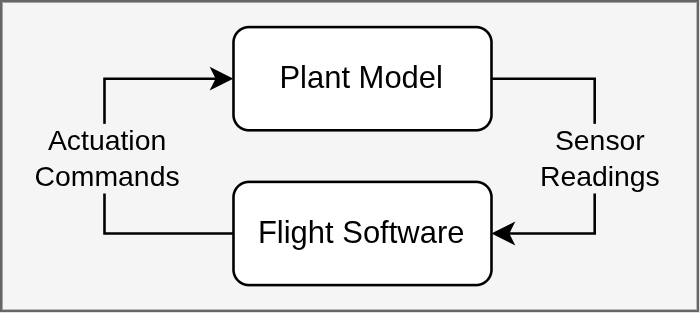
\includegraphics[width=0.5\textwidth]{figures/simulation verification.drawio.png}
    \caption{Closed-loop simulation-based verification, showing the data exchange between the plant model and flight software.}
    \label{fig:simulation-diagram}
\end{figure}


The fidelity of this approach depends on how closely the plant model captures the real vehicle's dynamics and on whether the software executes on a host machine or the actual flight hardware \cite{ulbig2019flightsimulatorbasedverification, kiesbye2019-moveII-cubsat}. Two methodologies reflect this tradeoff: Software-in-the-Loop (SIL) and Hardware-in-the-Loop (HIL).

In SIL testing, the system under test and the plant model are executing on the same host under common time \cite{ulbig2019flightsimulatorbasedverification}. This makes SIL fast to set up and well-suited to early development, where the goal is to validate software logic before committing to hardware. In HIL testing, the flight software is deployed and executed on the actual target hardware, while the plant model continues to run on a separate host machine~\cite{kiesbye2019-moveII-cubsat, santos-hil-uav-autopilot}. Sensor data is transmitted to the hardware, and control outputs are returned over a physical interface, introducing real-time behaviour, latency and hardware-specific execution constraints that SIL cannot capture. This makes HIL a higher-fidelity verification step, confirming that the software behaves correctly not just in logic but under the timing and resource constraints of the real flight hardware.



\subsection{Co-Simulation}
Co-Simulation encompasses the theory and techniques for coupling independent simulators, each advancing its own internal state, to achieve a global simulation \cite{gomes2017cosimulation}. Each simulator acts as a black box, interacting only through exchanges of inputs and outputs at synchronisation points separated by a communication step size $H$ \cite{gomes2017cosimulation}.

Simulators in Co-Simulation theory may be continuous-time, integrating a set of differential equations internally between communication steps, or discrete, advancing only when triggered by an external event \cite{gomes2017cosimulation}.  This distinction is central to the coupling problem addressed in this thesis. RocketPy is a continuous-time simulator, while F Prime flight software executes as a discrete, event-driven process. The way the two are coupled at their synchronisation boundary is described in Section~\ref{closed-loop-sim-env}.



\section{Related Work}\label{s:related}
Simulation-based testing is standard practice in the aerospace sector, where real flight tests are expensive, risky, and difficult to repeat under controlled conditions~\cite{bittar-guidance-sil-uav-xplane-simulink, santos-hil-uav-autopilot}. The dominant approach couples flight software with a physics-based simulator, exchanging states throughout the simulation. This pattern is particularly well-established in the Unmanned Aerial Vehicle (UAV) sector. 

Santos et al.~\cite{santos-hil-uav-autopilot} built an HIL environment that couples a PC flight simulator, X-Plane, with a dedicated microcontroller running a full lateral and longitudinal autopilot. Since X-Plane operates natively in real time, the two systems run independently, communicating over Ethernet using UDP at 20 Hz. Santos et al. validated the HIL framework by testing longitudinal and lateral control loops on a PT-60 radio-controlled aircraft model in X-Plane. Both control loops within the framework achieved the desired altitude and roll behaviour throughout the respective operations. The findings of their study confirm that the HIL environment is sufficient for developing and tuning control parameters without physically flying the aircraft and risking the airframe during testing.


% For the longitudinal axis, the autopilot was commanded to climb from an initial altitude to 3000ft, then to 5000ft. In both cases, it reached the desired altitude and demonstrated a stable level flight. For the lateral axis, the autopilot was commanded to change heading from 120\degree~to 200\degree~, and achieved stable roll behaviour throughout the operation. 


Bittar et al.~\cite{bittar-guidance-sil-uav-xplane-simulink} follow the same pattern, but transition to a SIL context, coupling X-Plane as the flight dynamics simulator with Simulink executing the control algorithms, communicating over UDP at 20Hz, on the same machine. These studies show that this independent-process pattern holds regardless of whether flight software runs on dedicated hardware or on a host computer.

% \begin{figure}[h]
%     \centering
%     \includegraphics[width=0.75\linewidth]{figures/lit_review/matlab-xplane-bittar.png}
%     \caption{SIL architecture showcasing Simulink executing the guidance and control algorithms while X-Plane handles the vehicle dynamics, with state exchanged over UDP. Reproduced from Bittar et al.~\cite{bittar-guidance-sil-uav-xplane-simulink}.}
%     \label{fig:matlab-xplane-bittar}
% \end{figure}

Coopmans et al.~\cite{coopmans-sil-hil-verification-uav} further validate that simulated UAV trajectories using SIL and HIL setups closely match real flight data. The authors demonstrate this using JSBSim as the flight simulator and the open-source Paparazzi autopilot as the flight software. In SIL mode, the Paparazzi control code is compiled and executed on a laptop against the JSBSim model, without additional hardware required. In HIL mode, the same code runs unchanged on the actual autopilot hardware, with JSBSim providing simulated sensor input through a serial driver in place of physical sensors. In their tests, the flight plan remained the same across all three modes: SIL, HIL and real flight, enabling a direct comparison. All three modes produced similar trajectories, remaining within 10\% error despite 6~$m/s$ wind conditions, leading the authors to conclude that both SIL and HIL are sufficiently accurate for rapid development and tuning of control parameters.

% \begin{figure}[h]
%     \centering
%     \includegraphics[width=0.75\linewidth]{figures/lit_review/figure-8-coopman.png}
%     \caption{UAV Trajectories of a figure-eight manoeuvre across SIL, HIL and real flight, demonstrating close agreement between all modes. Reproduced from Coopmans et al.~\cite{coopmans-sil-hil-verification-uav}.}
%     \label{fig:figure-8-coopman}
% \end{figure}

This pattern extends beyond UAVs to small spacecraft, a domain closer to the context of high-powered rockets addressed in this study. Kiesbye et al.~\cite{kiesbye2019-moveII-cubsat} developed a combined SIL and HIL environment for the MOVE-II CubeSat at the Technical University of Munich. The entire simulation, including the space environment, orbital dynamics, sensor models and actuator models, runs in Matlab/Simulink. In SIL mode, the attitude control algorithms are implemented in C++, embedded into the Simulink model as Level-2 S-functions, and executed within the simulation environment. In HIL mode, the flight code runs on the satellite hardware, with Simulink transmitting simulated sensor data via interface simulators over UDP, enabling communication with the hardware via its Serial Peripheral Interface (SPI) bus, and reading actuator commands back to close the loop. The authors demonstrate that this simulation environment supports the development and verification of MOVE-II's flight software throughout its mission, and continues to be used after launch to analyse in-flight issues and verify software updates before uplink. Notably, the SIL approach requires embedding flight logic as S-function blocks within Simulink, a constraint that does not extend to flight software frameworks such as Paparazzi and F Prime, which run as independent processes with their own threading models and inter-process communication.



The only published work connecting RocketPy to embedded hardware is Netzel et al. \cite{netzel-rocketpy-hil}, who validated their onboard flight software apogee detection algorithm by replaying pre-computed RocketPy trajectories as sensor data over SPI. While this confirms that the hardware correctly processes sensor readings, the approach is open-loop, as the simulation is pre-computed and not influenced by the outputs of the flight software. Control algorithms and recovery timing under dynamic flight conditions, therefore, cannot be validated using this method. RITL addresses this limitation directly by coupling RocketPy and F Prime in a live closed feedback loop, where actuation outputs influence the simulation state at each step.

These works establish simulation-based verification as a viable and well-validated approach for aerospace software, spanning UAV autopilots, CubeSat attitude control, and rocket apogee detection. However, none provides a closed-loop coupling framework between a high-powered rocketry trajectory simulator and a flight software framework. Existing HPR tools remain open-loop, and existing SIL/HIL frameworks are tightly coupled to specific simulation environments, such as Matlab/Simulink. RITL addresses this gap by coupling RocketPy with F Prime in a closed feedback loop, supporting SIL and HIL execution and enabling fault injection within the simulation loop.




\section{Closed-Loop Simulation Environment} \label{closed-loop-sim-env}%\label{s:overview}

% say we are addressing RQ 1 in the beginning

RocketPy is inherently a continuous-time simulator as it integrates a set of differential equations to propagate the rocket's trajectory. However, its implementation exposes a unique callback interface described in Section \ref{background-rocketpy}. While not designed for co-simulation, it can be repurposed as a synchronisation point that exchanges state with an external component at each discrete step. This is one of the key observations that drives this study, as it paves the way for coupling RocketPy with flight software in a closed-loop configuration.

In this study, the F Prime flight software is configured to perform three control tasks: deploying air brakes during the coasting phase to reach a target apogee of 3000\,m, triggering the drogue parachute at apogee and deploying the main parachute during descent. 

The following sections describe the simulation environment. Section~\ref{framework-arch} provides an overview of the architecture, introducing the three modules of the framework and the communication layer among them. Section \ref{s:fsw-arch} presents the flight software architecture, while Sections~\ref{lockstep}, \ref{snapshot}, and \ref{rate-group} detail each of the three coupling architectures evaluated in this study. Collectively, these sections answer RQ1 by documenting design and implementation decisions that support a closed-loop simulation environment involving RocketPy and F Prime.

\subsection{Framework Architecture}\label{framework-arch}
The framework proposed in Figure \ref{fig:architecture-diagram} places an Orchestrator between RocketPy and the F Prime FSW, a decision motivated by co-simulation literature of a coordinating component driving the exchange between simulators~\cite{gomes2017cosimulation}. Unlike a typical co-simulation coordinator, however, this Orchestrator does not control simulated time progression. RocketPy, instead, owns the simulation time internally via its integrator, while the Orchestrator is only invoked when RocketPy reaches a scheduled controller callback, set to 10Hz. To force the integrator to stop exactly at each scheduled node rather than stepping past it, \texttt{time\_overshoot} is disabled. RocketPy exposes four separate timing parameters relevant to this framework: the controller callback sampling rate described above, the sampling rate of RocketPy's built-in sensor models (accelerometer, barometer, gyroscope), the sampling rate of the drogue and main callback functions, and the solver's internal integration time step (\texttt{min\_time\_step} and \texttt{max\_time\_step}). These can, in principle, be set independently of one another.

Retaining the Orchestrator as a mediator, despite its non-compliance with strict co-simulation, offers two practical advantages. First, it decouples the interface from both the simulator and the flight software, meaning that either could be replaced without changes to the other. Second, it provides a natural point at which to apply additional processing, such as fault injection, before the sensor data is forwarded to the flight software.

To support fault injection, the Orchestrator includes a \texttt{FaultInjector} module that intercepts sensor data before it is forwarded to the FSW. This module has the opportunity to inject several faults to the outgoing sensor packets. In this study, a single fault is evaluated: a barometric freeze, where the barometric pressure reading is captured and held constant for all following packets. This allows failure-recovery behaviour to be tested within the same closed-loop configuration, without modifications to either RocketPy or the flight software.

\begin{figure}[h]
    \centering
    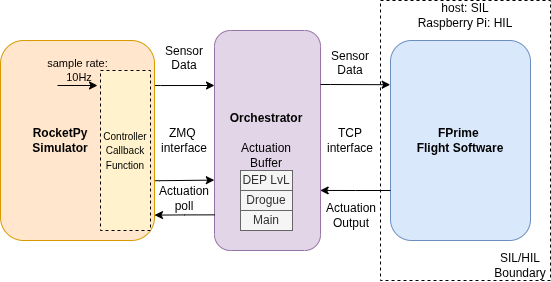
\includegraphics[width=0.5\textwidth]{figures/arch.png}
    \caption{The simulation architecture, consisting of the RocketPy simulator, the Orchestrator and the F Prime flight software.}
    \label{fig:architecture-diagram}
\end{figure}

\subsubsection{Communication Layer}
ZMQ was selected as the communication layer between RocketPy and the Orchestrator for two reasons. First, it is language agnostic, allowing the orchestrator interface to be used with simulators written in languages other than Python. Second, when both processes run on the same machine, ZMQ communicates via shared memory rather than the network stack, minimising communication overhead in SIL configurations. On the F Prime side, TCP was chosen over UDP for two reasons. First, one of the coupling strategies evaluated (Lockstep, introduced in Section \ref{lockstep}) requires reliable and ordered delivery. Second, the same deployment communicates over the local loopback interface in SIL and over a physical Ethernet link in HIL with no changes required to the communication layer. The trade-off is that TCP introduces connection overhead that UDP would avoid. 

\subsubsection{Sensor Data Flow}
In each controller callback function, RocketPy-simulated sensor readings are passed to the Orchestrator via ZMQ. Sensor data consists of accelerometer, gyroscope, and barometer readings, taken from RocketPy's sensor models along with the current simulation time $t$. The Orchestrator then forwards these readings directly to F Prime over TCP, where they are received by the flight software as if received from physical sensors.


\subsubsection{Actuation Data Flow}

The return path is more constrained. RocketPy's controller callback expects a synchronous return value, as there is no mechanism to send a control command to the simulation while it is running. The Orchestrator, therefore, maintains a buffer of the last known actuation output received from F Prime, consisting of the air brake deployment level, a continuous value in the range $[0,1]$ and two boolean deployment flags for the drogue and main parachutes. How the Orchestrator uses this buffer at callback time depends on the coupling strategy, as described in Sections~\ref{lockstep} -- \ref{rate-group}.


\subsubsection{SIL/HIL Capabilities}
The framework supports SIL and HIL execution without changes to Orchestrator or RocketPy. In SIL, F Prime runs as a native process on the same host machine, with TCP communication over the local loopback interface. In HIL, the same F Prime deployment is cross-compiled for the Raspberry Pi, with TCP communication routed over a physical Ethernet Link. The only change required is pointing the Orchestrator at the FSW's IP and port. A second capability comes from F Prime's topology abstraction. Since a topology is just a declarative wiring of components, different topologies can be defined for different flight computer architectures without changing the underlying framework. This same abstraction also supports separate topologies for simulation and for actual flight. For instance, both topologies would share the same logic components but swap out the sensor components, where the flight topology reads from physical sensors, while the simulation topology reads from the Orchestrator via the same interface.



\subsection{Flight Software Architecture}\label{s:fsw-arch}
The fidelity of the SIL and HIL configurations depends on the flight software as much as on the simulation infrastructure. The deployment architected in this study mirrors a real avionics system, replacing only the hardware drivers with simulated counterparts.

\begin{figure}[h]
    \centering
    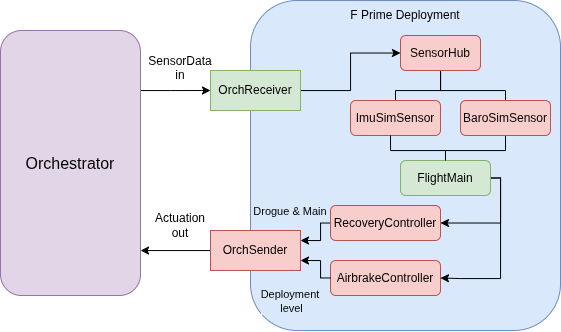
\includegraphics[width=0.5\textwidth]{figures/fsw-arch.png}
\caption{General FSW architecture. Components are coloured 
by execution type: green for active, red for passive.}
    \label{fig:fsw_architecture-diagram}
\end{figure}

The proposed FSW architecture is illustrated in Figure~\ref{fig:fsw_architecture-diagram}. Component colours indicate execution type specific to F Prime: green for active, red for passive. Communication with the Orchestrator is handled by two dedicated components: \texttt{OrchReceiver}, a TCP client that receives incoming sensor data, and \texttt{OrchSender}, a TCP server that transmits actuation outputs back to the Orchestrator. 

Incoming sensor data is distributed via the \texttt{SensorHub}. This component holds the data packet as it arrives from the Orchestrator, including the simulation time $t$. The \texttt{SensorHub} distributes sensor data to its respective sim sensor components, \texttt{ImuSimSensor} and \texttt{BaroSimSensor}, which repackage accelerometer/gyroscope and barometer readings into the port types expected by the flight logic. This abstraction mirrors real flight software, where \texttt{FlightMain} reads from the same sensor interfaces regardless of whether the source is simulated or physical hardware. These SimSensors are present in the Figure but are only active in the clock-driven topology, as described in Section~\ref{fsw-exec-topologies}.


\texttt{FlightMain} is the central flight logic component. It is responsible for phase detection and sending control outputs. It delegates air brake control to \texttt{AirbrakeController}, which computes the deployment level during the coasting phase, and to \texttt{RecoveryController} for parachute deployment actuations.


\subsubsection{FSW Execution Topologies} \label{fsw-exec-topologies}
During the implementation of the flight software, two execution topologies emerged as fitting for the coupling strategies under evaluation. This split reflects a long-standing distinction in real-time systems between time-triggered and event-triggered architectures~\cite{scheler-time-trigger-event-trigger}. In a time-triggered system, activities are executed periodically at predetermined points regardless of external events. In contrast, in an event-triggered system, execution is initiated directly by the occurrence of a signal or event. In this study, the clock-driven topology corresponds to the time-triggered model, while the sensor-driven topology corresponds to the event-triggered model. Both are illustrated in Figures~\ref{fig:clock-driven-arch-diagram} and~\ref{fig:sensor-driven-arch-diagram}. The choice of topology for a given coupling strategy is described in Sections~\ref{lockstep}--\ref{rate-group}.


The clock-driven topology illustrated in Figure \ref{fig:clock-driven-arch-diagram} decouples data arrival from FSW execution. \texttt{OrchReceiver} runs on its own thread, continuously receiving sensor packets and updating \texttt{ImuSimSensor} and \texttt{BaroSimSensor} buffers via the \texttt{SensorHub}. \texttt{FlightMain} is driven independently by a \texttt{LinuxTimer}, which ticks a passive \texttt{RateGroupDriver} at a configurable frequency. On each tick, \texttt{FlightMain} polls the latest available values from these buffers, regardless of when the last packet arrived. This topology mirrors real flight software more closely, where the avionics loop runs on a fixed schedule driven by a hardware timer, and sensor reads are decoupled from the arrival of new data.

\begin{figure}[h]
    \centering
    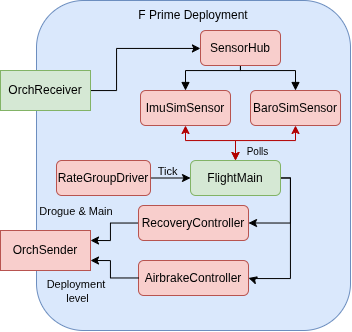
\includegraphics[width=0.4\textwidth]{figures/rate-group-arch.png}
   \caption{The clock-driven topology. \texttt{FlightMain} 
is driven by a \texttt{LinuxTimer} at a configurable frequency, reading sensor data from the SimSensor buffers on each tick.}
    \label{fig:clock-driven-arch-diagram}
\end{figure}

The sensor-driven topology, illustrated in Figure~\ref{fig:sensor-driven-arch-diagram}, removes this decoupling. Both \texttt{OrchReceiver}  and \texttt{FlightMain} are active components, each running on its own thread. \texttt{OrchReceiver} continuously listens for incoming sensor packets and, upon receipt, forwards them to \texttt{SensorHub}, which passes the data packet directly to \texttt{FlightMain}'s message queue. Unlike clock-driven topology, \texttt{ImuSimSensor} and \texttt{BaroSimSensor} are absent, as the incoming sensor packet is itself the tick that drives \texttt{FlightMain}, so there is no intermediate state to hold. This makes the execution order deterministic with respect to sensor arrival, since \texttt{FlightMain} always processes each packet directly rather than polling a buffer that may or may not have been updated since the last tick.



\begin{figure}[h]
    \centering
    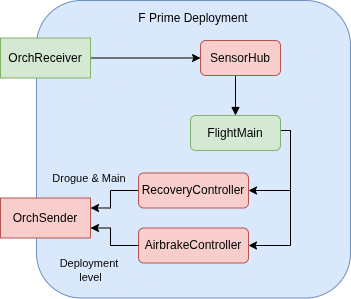
\includegraphics[width=0.4\textwidth]{figures/sensor-driven-arch.png}
    \caption{The sensor-driven topology, in which \texttt{OrchReceiver} triggers \texttt{FlightMain} directly on each incoming sensor packet.}
    \label{fig:sensor-driven-arch-diagram}
\end{figure}

\subsubsection{Flight Logic} \label{flight-logic}
The flight software implements two independent controllers invoked from \texttt{FlightMain}: \texttt{AirbrakeController}, which manages drag control during the coasting phase via a PI controller, and \texttt{RecoveryController}, which handles parachute deployment via apogee detection.

\texttt{AirbrakeController} activates after motor burnout. Burnout is detected when the vertical acceleration from the IMU drops below 15 $m/s^2$ following a period of sustained positive thrust. During the coasting phase, the controller estimates the predicted apogee as follows:

\begin{equation}
\hat{a} = h + \frac{v_z^2}{2g}
\end{equation}

\noindent where $g = 9.81\,\text{m/s}^2$, $v_z$ is the vertical velocity integrated from IMU acceleration readings, and $h$ is the barometric altitude derived from the International Standard Atmosphere model:

\begin{equation}
    h = 44330 \left(1 - \left(\frac{P}{P_0}\right)^{\frac{1}{5.255}}\right)
    \label{eq:baro}
\end{equation}

\noindent where $P$ is the current barometric pressure and $P_0$ is the reference pressure at the ground level that is recorded from the first reading of the flight software at initialisation.

A PI controller commands the airbrake deployment. The proportional term responds to the difference between $\hat{a}$ and the target apogee 3000~m, whereas the integral term accumulates this error over time. The air brake deployment level is clamped to $[0, 1]$ as required by RocketPy, and an anti-wind-up clamp bounds the integral term to prevent integrator saturation during extended coasting. The controller deactivates once 10 consecutive barometric readings indicate a decreasing altitude, at which point the air brakes are fully retracted. The controller constants were selected to produce stable, non-oscillatory actuation toward the 3000\,m target. Formal tuning is outside the scope of this study.

\texttt{RecoveryController} detects apogee using barometric pressure. Multiple apogee detection approaches exist, including IMU-based velocity integration and Kalman filters \cite{kimani2022detection}. Barometric detection was chosen for its simplicity, as flight logic implementation is not the focus of this study. The implementation tracks the minimum observed pressure and fires the drogue parachute only after 10 consecutive readings exceed that minimum by 0.5 hPa. The main parachute is deployed when the pressure has increased by 40 hPa above the recorded apogee minimum, corresponding to a descent of approximately 330 m under the ISA model.

The \texttt{RecoveryController} component facilitates the testing of failure-recovery behaviour by implementing fallback logic for cases where barometric readings are not reliable. If consecutive barometer readings become stale, differing by less than \texttt{BARO\_FREEZE\_DELTA} for \texttt{BARO\_FREEZE\_COUNT} samples after launch, the controller detects a sensor fault and switches to IMU-based apogee detection. The drogue deployment is then activated when the magnitude of the vertical IMU acceleration drops below \texttt{ACCEL\_FREEFALL\_THRESH}, indicating that the rocket has entered free fall. If the fault persists after drogue deployment, the main parachute is deployed after a fixed timeout of \texttt{MAIN\_DEPLOY\_TIMEOUT} rather than waiting for the pressure-based threshold. The constants governing both controllers are summarised in Table~\ref{tab:controller-constants}.


\begin{table}[h]
\centering

\small
\begin{tabular}{llp{3.8cm}}
\toprule
\textbf{Constant} & \textbf{Value} & \textbf{Description} \\
\midrule
\texttt{TARGET\_APOGEE}            & 3000\,m        & PI target \\
\texttt{Kp}                        & 0.001          & Proportional gain \\
\texttt{Ki}                        & 0.0001         & Integral gain \\
\texttt{INTEGRAL\_CLAMP}           & 1000           & Anti-windup bound \\
\texttt{BOOST\_ACCEL\_THRESHOLD}   & 15\,m/s$^2$    & Burnout threshold \\
\texttt{DESCENT\_COUNT\_THRESHOLD} & 10             & Descent readings to retract \\
\texttt{APOGEE\_BARO\_DELTA}       & 0.5\,hPa       & Pressure rise per confirmation \\
\texttt{APOGEE\_CONFIRM\_COUNT}    & 10              & Confirmations before drogue \\
\texttt{MAIN\_DEPLOY\_DELTA\_HPA}  & 40\,hPa        & Pressure rise for main deployment \\
\texttt{BARO\_FREEZE\_DELTA}       & 1\,hPa         & Max variation for freeze detection \\
\texttt{BARO\_FREEZE\_COUNT}       & 15             & Frozen samples before fault \\
\texttt{LAUNCH\_ACCEL\_THRESH}     & 20\,m/s$^2$    & Launch detection threshold \\
\texttt{ACCEL\_FREEFALL\_THRESH}   & 2\,m/s$^2$     & Free-fall detection threshold \\
\texttt{MAIN\_DEPLOY\_TIMEOUT}     & 20\,s          & Fallback main deploy timeout \\
\bottomrule
\end{tabular}
\caption{Constants for \texttt{AirbrakeController} and \texttt{RecoveryController}.}
\label{tab:controller-constants}
\end{table}

\subsection{Lockstep Strategy } \label{lockstep}
The Lockstep Strategy is the most tightly synchronised of the three coupling architectures evaluated in this study. It uses the sensor-driven topology described in Section~\ref{fsw-exec-topologies}. After sending the sensor data to the FSW, the Orchestrator blocks on the TCP connection, waiting for an actuation response before returning from the callback. This guarantees that every simulation step is computed using the actuation output corresponding to that exact sensor reading, meaning there is no lag between the plant model and the control output. This makes Lockstep the appropriate choice when the goal is to isolate the correctness of the flight logic itself, since eliminating timing effects removes any ambiguity between a logic error and one of execution timing.



% The cost is wall-clock time, as the simulation idles at every callback until the flight software responds.

\subsection{Snapshot Strategy}\label{snapshot}
The Snapshot strategy relaxes the synchronisation constraint of Lockstep. It also uses the sensor-driven topology, but the Orchestrator does not block after sending the sensor packet. Instead, it immediately returns the latest values in the Actuation Buffer to RocketPy and continues. \texttt{FlightMain} still processes each sensor packet, but its actuation response updates the buffer only after RocketPy has already advanced to the next step, which means that the simulation continues using the actuation from the previous tick. This reduces wall-clock time by eliminating the blocking wait, at the cost of a looser coupling between the plant state and the control output.

\subsection{Rate Group Strategy}\label{rate-group}
The Rate Group Strategy completely decouples flight software execution from the RocketPy callback. It uses the clock-driven topology, where \texttt{FlightMain} runs on a fixed hardware timer, independent of when the callback fires. The Orchestrator behaves identically to Snapshot, forwarding sensor packets and returning the latest actuation buffer value without blocking. The actuation buffer reflects whatever the FSW last computed, which may have been on a different tick from the current callback. This is the closest of the three strategies to real flight software behaviour, where the FSW loop runs on a hardware-driven schedule, independent of any external synchronisation. The trade-off is timing non-determinism, since the FSW and RocketPy run on independent clocks, the values in the actuation buffer at any given callback may have been computed on a different tick, introducing variability in control output timing. This same non-determinism makes the Rate Group strategy the hardest of the three strategies to use for isolating flight logic errors.

Together, the three strategies span a spectrum from fully synchronised to fully decoupled and are evaluated experimentally in Section \ref{experiment-design}.




% \TODO{
% This section provides a high-level outline of the proposed system or solution.
% It typically illustrates the system architecture or the interactions between the
% different solution components (via a ``boxes-and-arrows'' diagram) from a user’s
% perspective.
% }



\section{Experimental Design}\label{experiment-design}
\textbf{Hypotheses.} $H_1$: strategies that decouple the FSW from each simulation step delay actuation and so overshoot the standalone baseline apogee, while Lockstep does not. $H_2$: HIL runs take longer in wall-clock time than SIL runs, because of Ethernet latency and the slower CPU. $H_3$: after a barometer freeze injected mid-flight, the FSW detects the fault and deploys the drogue near apogee through the IMU fallback, in both SIL and HIL. $H_1$ and $H_2$ address RQ2, and $H_3$ addresses RQ3.

\textbf{Rocket and baseline.} We use the Camões rocket, built by Rocket Experiment Division and launched at EuRoC 2023 (recorded apogee 3015\,m, RocketPy prediction 3003\,m), configured from RocketPy's public example~\cite{rocketpy_camoes}. That example computes actuation directly from the ground-truth state vector, which an embedded FSW never has, so its flight logic cannot be reused. We wrote the flight logic of Section~\ref{flight-logic} instead. The baseline is a standalone RocketPy simulation with the same rocket, motor and environment, in which that logic is translated to Python and runs inside the callback on RocketPy's sensor models. Any difference between baseline and RITL therefore comes from the coupling alone. The baseline has no networked or hardware components, so its apogee and event times are deterministic; only its wall-clock time varies.

\textbf{Variables.} We vary the coupling strategy, the execution context (SIL or HIL), the \texttt{RateGroupDriver} tick frequency (1, 5, 10, 25 and 50\,Hz, Rate Group only) and the controller callback rate (5, 10, 25, 35 and 50\,Hz, baseline, Lockstep and Snapshot only). The dependent variables are apogee altitude and time, drogue and main deployment times, and wall-clock time per run. Unless varied, the sensor-model rate, the parachute-trigger rate and the controller callback rate are fixed at 10\,Hz and the solver step at 0.001\,s.

\textbf{Experiments.} We automate 10 runs per configuration (unless stated otherwise) with the experiment runner of Karsten et al.~\cite{karsten2026experiment-runner}.
(1)~\emph{Coupling comparison:} all three strategies in SIL and HIL, with Rate Group at 25\,Hz, chosen from the sweep.
(2)~\emph{Rate Group sweep:} 1--50\,Hz in SIL and HIL.
(3)~\emph{Fault injection:} the \texttt{FaultInjector} freezes the barometer at $t=10$\,s, during the coast after burnout and before apogee, with the Snapshot strategy as a middle ground, in SIL and HIL.
(4)~\emph{Callback-rate sweep:} the controller callback rate is varied for the baseline, Lockstep and Snapshot. Rate Group is excluded, since its FSW rate is set by the tick frequency. A brief solver-step check runs the baseline and Snapshot at steps of 0.001, 0.005, 0.01 and 0.0001\,s, one run each, because the check is exploratory and the finest step is expensive.
SIL runs on a laptop (Intel Core Ultra 7 155H, 32\,GiB, Pop!\_OS 22.04). HIL runs on a Raspberry Pi 4B (Cortex-A72, 8\,GiB, Raspberry Pi OS) connected to the host by a direct Ethernet link. We compare each configuration against the baseline with a two-sample Welch $t$-test at $\alpha=0.05$. Because variance is low in most conditions, we interpret accuracy against the 12\,m threshold.

\section{Results and Discussion}\label{s:evaluation}
This section reports the interpretation of the experimental results addressing RQ2 and RQ3, evaluated against the hypotheses $H_1$-- $H_3$ defined in Section~\ref{hypotheses}. Standard deviations are reported throughout to characterise the run variability introduced by each coupling strategy. Statistical significance is assessed using a two-sample Welch t-test at $\alpha$ = 0.05. Given the low variance observed in most conditions, the 12\,m acceptance threshold defined in Section~\ref{ss:rqs} is used as the primary basis for interpreting accuracy, with significance testing confirming that observed differences are not attributable to sampling noise.
 

\subsection{Coupling Strategy Comparison and One-Tick Delay Analysis}\label{coupling-results}


Table~\ref{tab:summary} reports the mean apogee height and time as well as wall-clock time over 10 runs per strategy, relative to the RocketPy standalone baseline. 


\begin{table}[h]
\centering
\small
\begin{tabular}{lrrr}
\toprule
\textbf{Mode} & \textbf{Apogee (m)} & \textbf{Apogee Time (s)} & \textbf{Wall Time (s)} \\
\midrule
Non-SIL (baseline)    & 3061.94 $\pm$ 0.00 & 23.49 & 27.0 $\pm$ 1.4 \\
\midrule
SIL Lockstep          & 3061.86 $\pm$ 0.04 & 23.45 & 44.9 $\pm$ 3.8 \\
SIL Snapshot          & 3065.98 $\pm$ 0.03 & 23.46 & 36.4 $\pm$ 2.0 \\
SIL Rate Group 25\,Hz & 3065.78 $\pm$ 0.19 & 23.46 & 36.0 $\pm$ 4.5 \\
\midrule
HIL Lockstep          & 3061.87 $\pm$ 0.03 & 23.45 & 48.8 $\pm$ 3.7 \\
HIL Snapshot          & 3066.00 $\pm$ 0.06 & 23.46 & 41.8 $\pm$ 1.3 \\
HIL Rate Group 25\,Hz & 3069.33 $\pm$ 7.46 & 23.48 & 38.2 $\pm$ 1.7 \\
\bottomrule
\end{tabular}
\caption{Mean apogee ($\pm$ 1 std dev), apogee time, and wall-clock time per coupling strategy, relative to the standalone RocketPy baseline of 3061.94\,m.}
\label{tab:summary}
\end{table}




% \begin{figure}[h]
%     \centering
%     \includegraphics[width=\columnwidth]{figures/results/apogee_bars.png}
%     \caption{Mean apogee per coupling strategy ($\pm$ 1 std dev) across ten runs, with the standalone RocketPy baseline shown as a dashed reference line.}
%     \label{fig:apogee_bars}
% \end{figure}

\subsubsection{Accuracy}
The Lockstep strategy produces the closest apogee to the baseline in both SIL and HIL contexts, with a mean of 3061.86\,m in SIL (-$0.08\,m, $p=0.0001) and 3061.87\,m in HIL (-$0.07\,m, $p=0.0001). Although both are statistically significant, the errors are practically negligible against the acceptance threshold of 12\,m. This is because Lockstep blocks the simulation at every callback until the FSW responds, ensuring that each simulation step uses the actuation output corresponding to the exact sensor reading. It represents an idealised synchronised model that does not exist in real hardware interacting with its environment, but it validates the correctness of flight logic under ideal conditions.

Snapshot produces a consistent overshoot at apogee with a mean of 3065.98\,m in SIL (+$4.04\,m, $p<0.001) and 3066.00\,m in HIL (+$4.06\,m, $p<0.001). The consistency of this overshoot is a structural property of the non-blocking orchestrator design. At callback $n$, the Orchestrator sends the current sensor packet to the FSW and immediately returns the actuation value computed at callback $n-1$ from the actuation buffer, without waiting for the FSW to process the packet from callback $n$. The actuation response corresponding to the callback $n$ is therefore not applied until the callback $n+1$, producing a one-tick delay, where the actuation applied at any callback is always one step behind the sensor reading that triggered it. This delay directly affects the \texttt{AirbrakeController}, as the predicted apogee estimate and the air brake deployment level are always one step behind the true simulation state, causing the PI controller to under-correct during the coasting phase and leading to a systematic overshoot.


The Rate Group strategy at 25Hz produces mean apogee of 3065.78\,m in SIL (+$3.84\,m, $p<0.001) and 3069.33\,m in HIL (+$7.39\,m, $p<0.001). The SIL result exhibits a similar baseline overshoot to Snapshot, consistent with both strategies sharing the same non-blocking simulation behaviour. Both Rate Group SIL and HIL apogee accuracy show higher variance than Snapshot, since \texttt{FlightMain} runs on its own independent clock, decoupled from RocketPy's callback function, meaning that the actuation buffer at any given callback may represent a value computed on a different tick. In HIL, this variance increases further, reaching 7.46\,m compared to 0.19\,m in SIL, as the difference between the two independent clocks compounds with the reduced CPU performance of the target hardware and added Ethernet latency. Together with the Lockstep and Snapshot results above, these findings confirm $H_1$, as Lockstep, which enforces synchronisation, produces negligible overshoot, while both non-blocking strategies, Snapshot and Rate Group, introduce a one-tick delay that causes a consistent apogee overshoot in both SIL and HIL.

All three strategies, however, remain within the 12 m acceptance threshold in both SIL and HIL, confirming that each is suitable for pre-flight validation despite their architectural differences.

The nature of this one-tick delay was further confirmed by running an informal check against a second rocket configuration (not part of the controlled experiments), in which the overshoot magnitude differed, but the delay persisted across both non-blocking strategies, confirming that it is a property of the Orchestrator design rather than the rocket configuration. The timing behaviour produced by this delay is representative of real embedded flight software execution. On real hardware, sensor readings will always be slightly stale by the time they are processed on a fixed hardware clock. 

Table~\ref{tab:deployment_timings} reports the parachute deployment times according to each strategy. Lockstep and Snapshot deploy the drogue at $t \approx 25.00$\,s across both SIL and HIL execution contexts, and the main parachute at $t \approx 44.60$\,s. The Rate Group strategy shows earlier drogue deployment at $24.84$\,s (SIL) and $24.91$\,s (HIL), but with higher variance in both drogue and main times consistent with its timing non-determinism.

\begin{table}[htbp]
\centering
\small
\begin{tabular}{lrrr}
\toprule
\textbf{Deployment} & \textbf{Drogue Parachute (s)} & \textbf{Main Parachute (s)} \\
\midrule
Non-SIL (baseline)   & $25.00 \pm 0.00$ & $44.60 \pm 0.00$ \\
\midrule
SIL Lockstep         & $25.00 \pm 0.00$ & $44.60 \pm 0.00$ \\
SIL Snapshot         & $25.00 \pm 0.01$ & $44.60 \pm 0.00$ \\
SIL Rate Group 25 Hz & $24.84 \pm 0.04$ & $45.18 \pm 0.25$ \\
\midrule
HIL Lockstep         & $25.01 \pm 0.00$ & $44.64 \pm 0.01$ \\
HIL Snapshot         & $25.01 \pm 0.00$ & $44.64 \pm 0.01$ \\
HIL Rate Group 25 Hz & $24.91 \pm 0.07$ & $45.09 \pm 0.28$ \\
\bottomrule
\end{tabular}
\caption{Mean parachute deployment timings and standard deviations per coupling strategy. Measured in simulation time $t$.}
\label{tab:deployment_timings}

\end{table}


\subsubsection{Wall-Clock Time}
Wall-clock time distributions are shown in Table \ref{tab:summary} and illustrated in Figure \ref{fig:wall_time_violin}. The stand-alone baseline completes in 27.0\,$\pm$\,1.4\,s, and all coupling strategies introduce overhead relative to it. Among SIL configurations, Lockstep is the slowest at 44.9\,$\pm$\,3.8\,s, while Snapshot and Rate Group are comparable at 36.4\,$\pm$\,2.0\,s and 36.0\,$\pm$\,4.5\,s, respectively. HIL configurations are slower than their SIL  counterparts across all strategies, with HIL Lockstep the slowest overall at 48.8\,$\pm$\,3.7\,s, followed by HIL Snapshot at 41.8\,$\pm$\,1.3\,s and HIL Rate Group at  38.2\,$\pm$\,1.7\,s.

\begin{figure}[h]
    \centering
    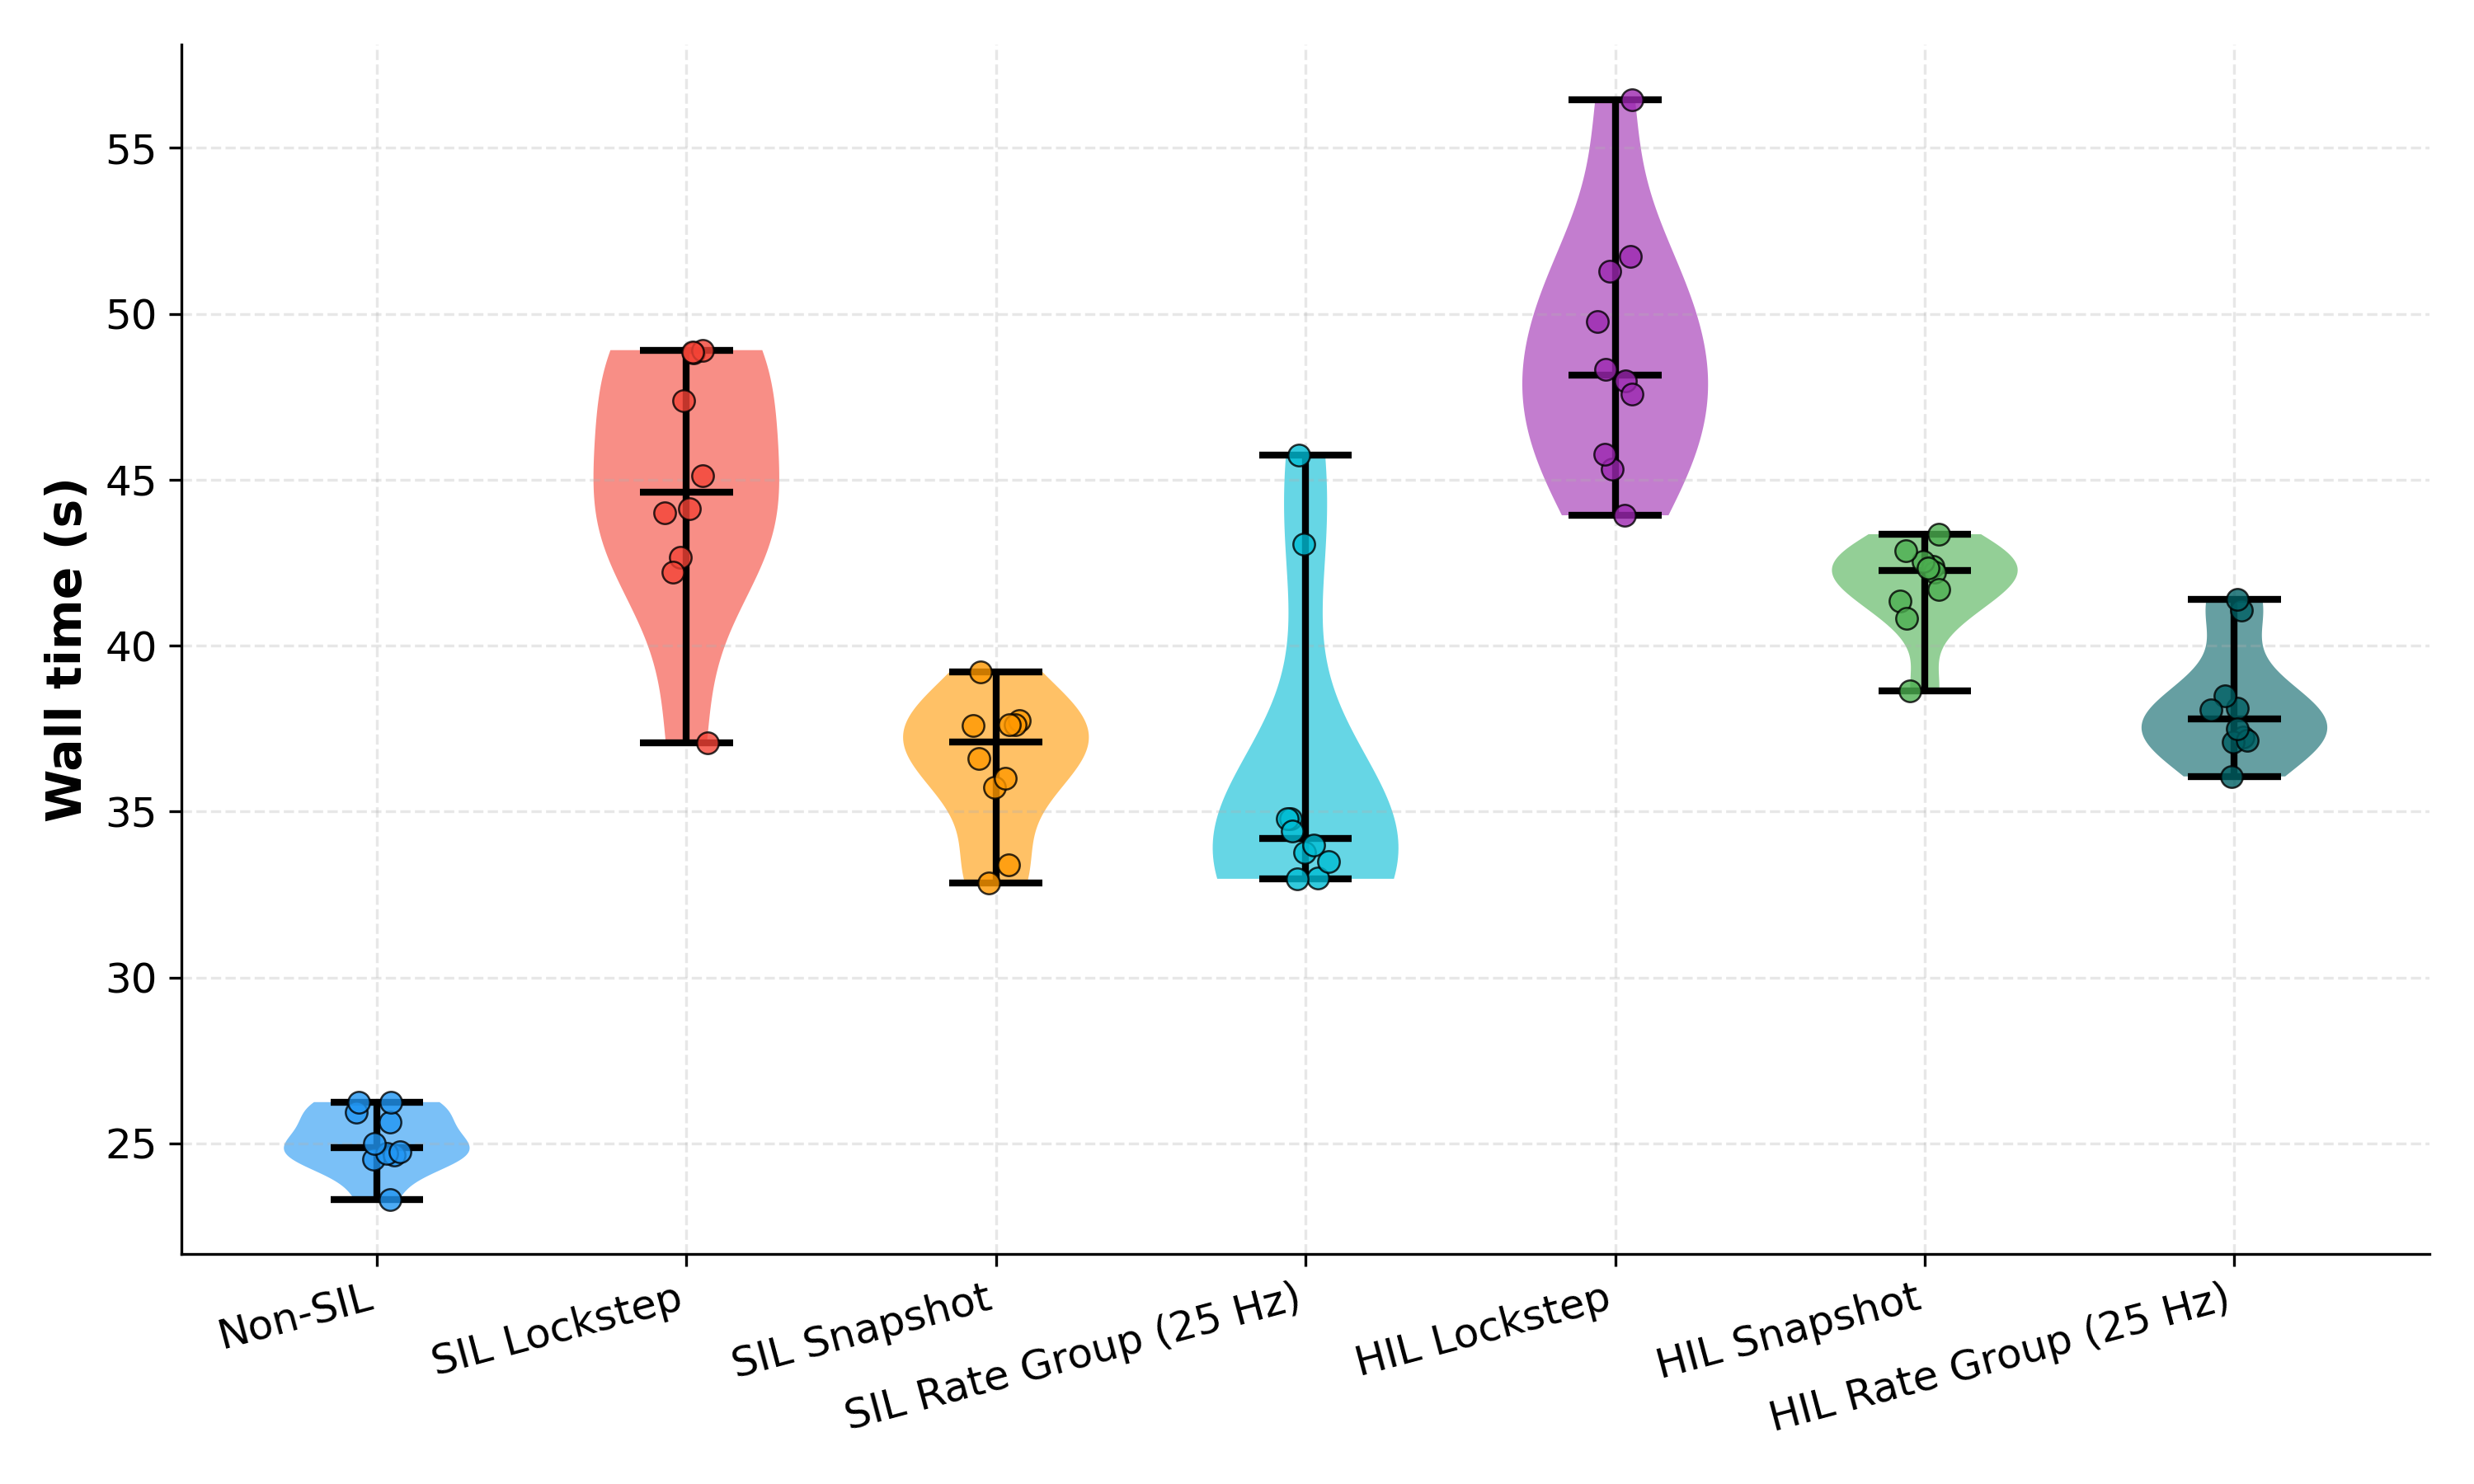
\includegraphics[width=\columnwidth]{figures/results/wall_time_violin.png}
    \caption{Wall-clock time distribution per coupling strategy.}
    \label{fig:wall_time_violin}
\end{figure}
For Lockstep, the overhead is most notable in both contexts due to its blocking nature. The additional cost in HIL relative to SIL (48.8\,s versus 44.9\,s) is attributed to the Ethernet round-trip between the host and the Raspberry Pi 4, as well as the reduced CPU performance of the target hardware, which extends the processing time of the FSW. For the Snapshot and Rate Group strategies, neither block the simulation, so the additional overhead is attributed to just the Ethernet transmission latency, as reflected in the smaller but consistent gap in wall-clock times. These results confirm $H_2$: HIL configurations produce longer wall-clock times than their SIL counterparts, attributable to Ethernet latency and reduced CPU performance on the target hardware.






% \subsection{SIL vs HIL Agreement}\label{sil-hil-results}

\subsection{Rate Group Frequency Sweep}\label{freq-sweep}
Figure~\ref{fig:rate-apogee-freq} shows the mean apogee as a function of \texttt{RateGroupDriver} tick frequency with SIL and HIL combined. At 1Hz, the mean apogee reaches 3271.5\,$\pm$\,59.0\,m; this is an overshoot of 209.56\,m, as the FSW uses stale data and transmits air brake actuations only once per second, too infrequently to efficiently track the coasting dynamics. A clear trend is evident: the error decreases monotonically with frequency, from 101.19\,m at 5\,Hz, to 27.69\,m at 10\,Hz, to 5.61\,m at 25\,Hz, to 4.0\,m at 50\,Hz. This is because at higher tick frequencies, the FSW reads more recent sensor data and actuates more frequently, reducing the window of stale data between ticks and allowing the \texttt{AirbrakeController} to track the trajectory with higher accuracy. The diminishing accuracy gains beyond 25\,Hz informed the selection of this frequency for the comparison of coupling strategies in Section~\ref{coupling-results}.

\begin{figure}[h]
    \centering
    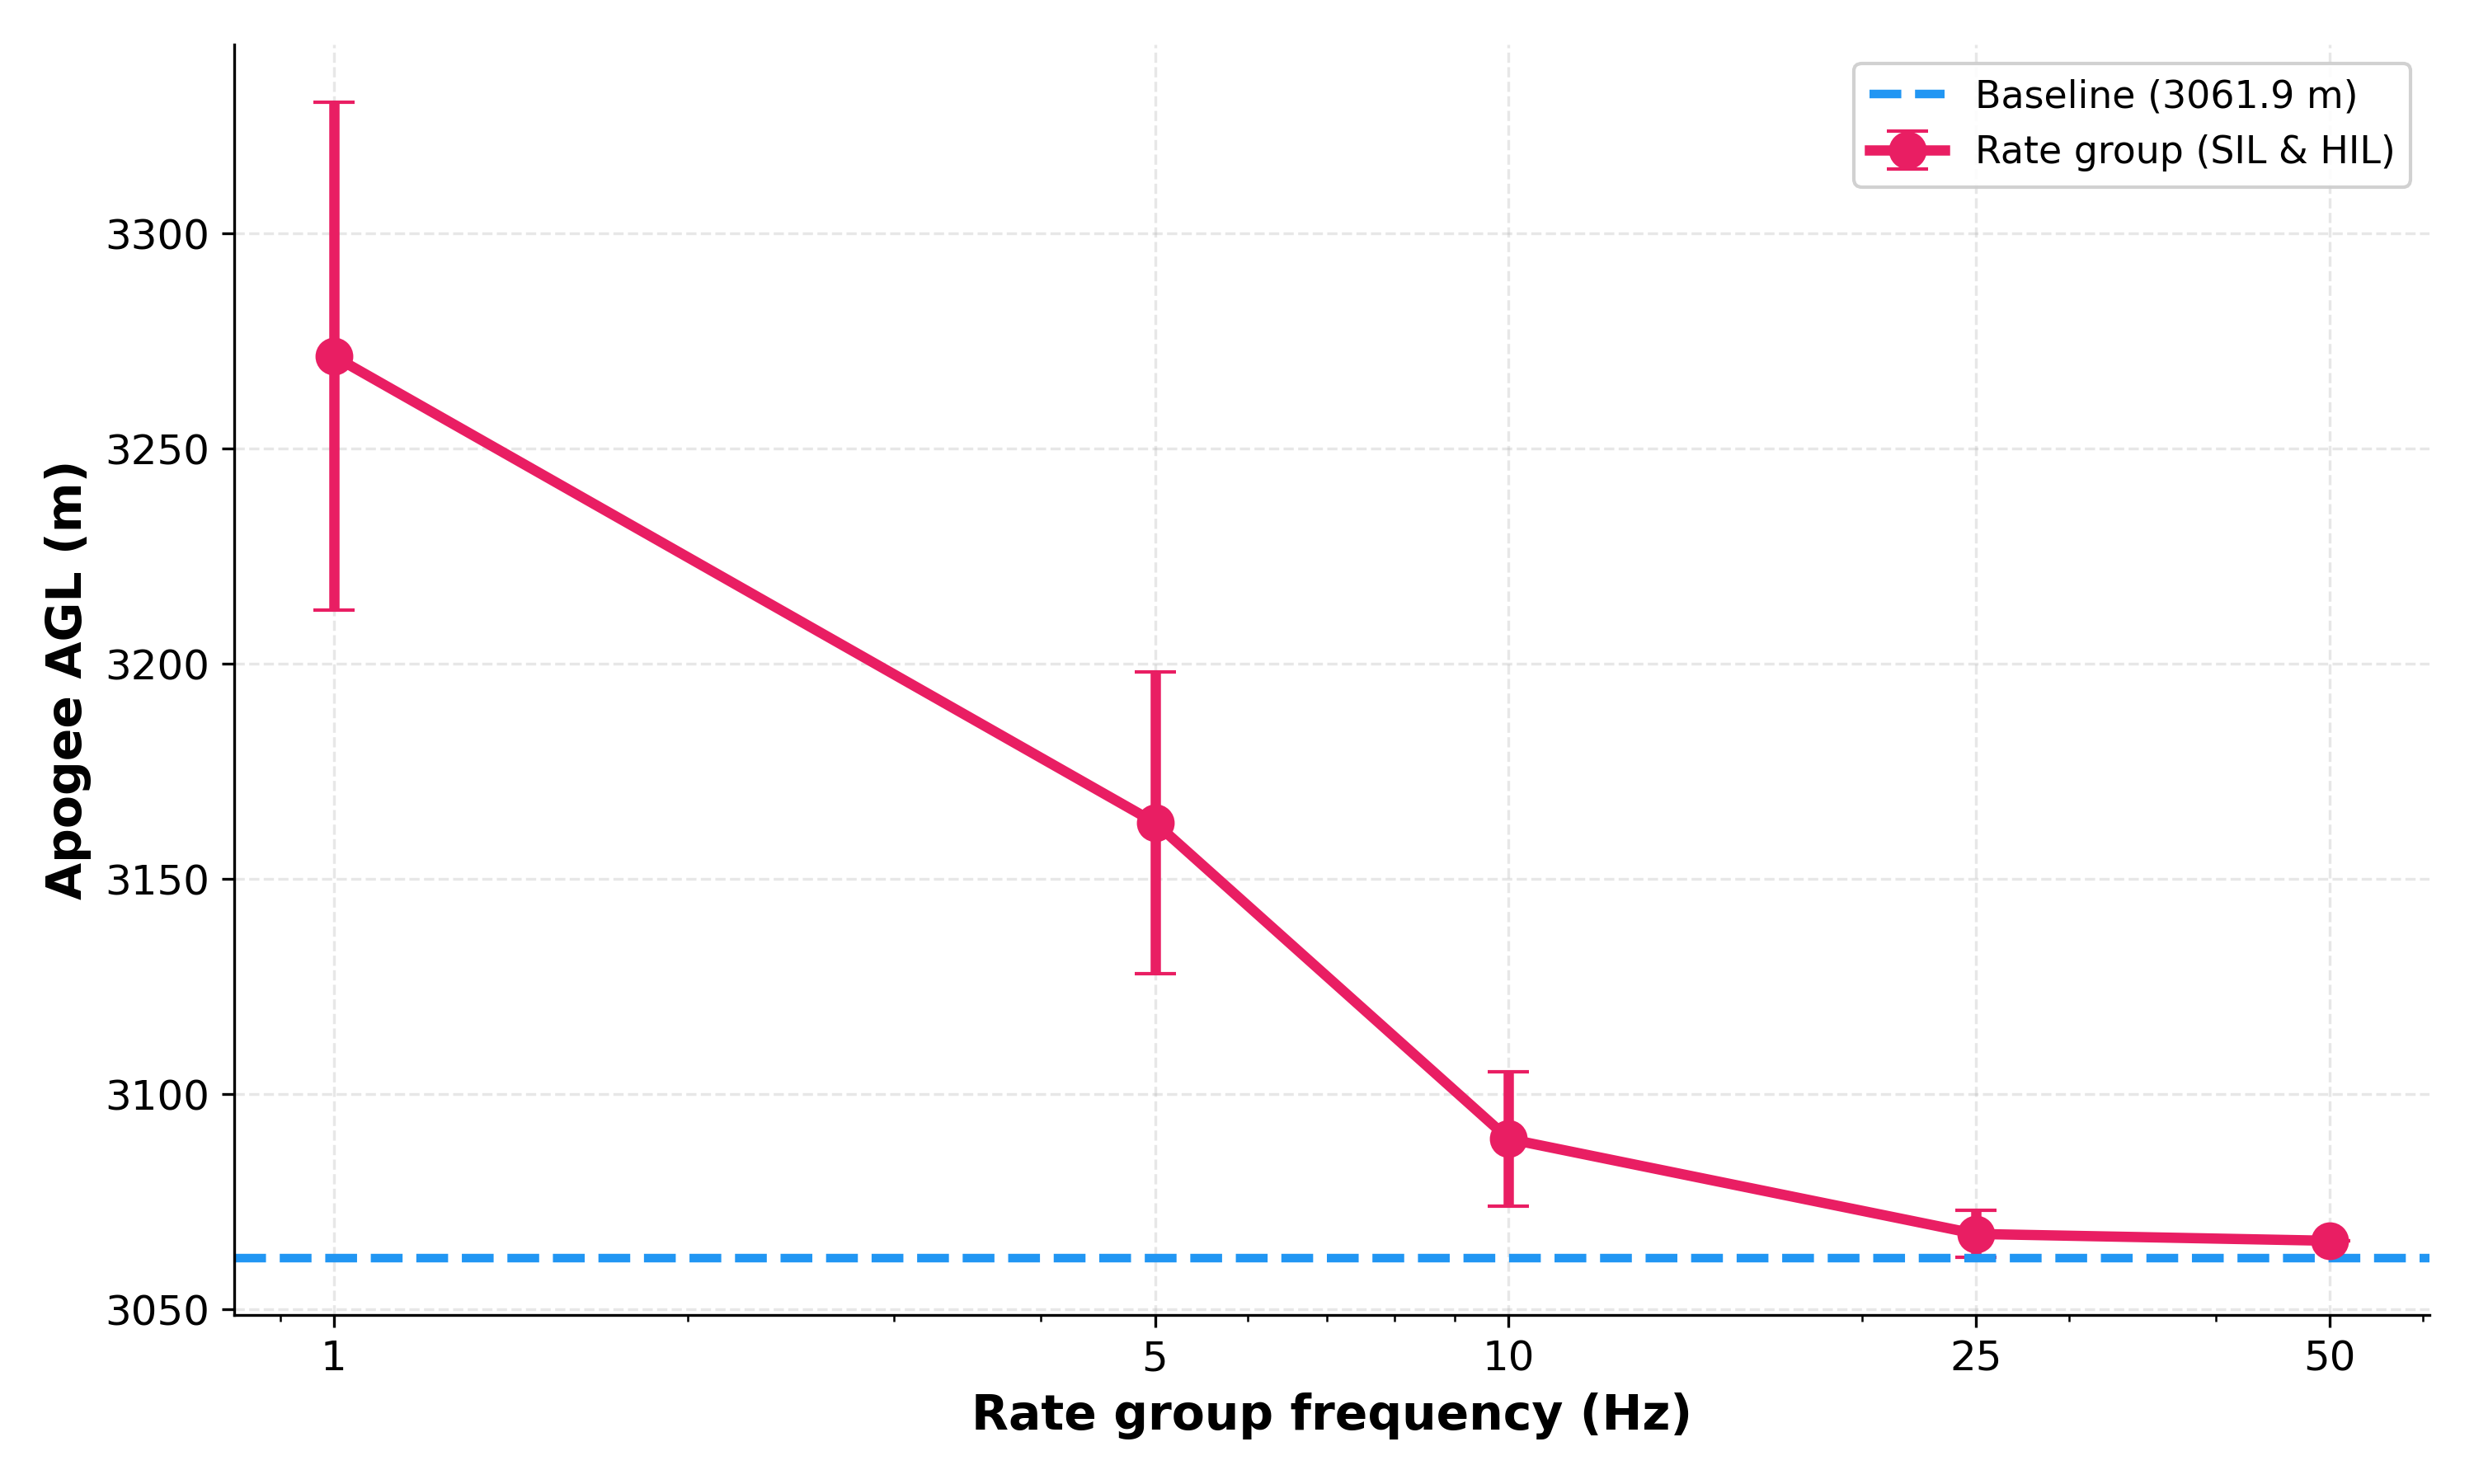
\includegraphics[width=\columnwidth]{figures/results/rategroup_apogee_vs_freq.png}
    \caption{Mean apogee as a function of Rate Group tick frequency, SIL and HIL combined.}
    \label{fig:rate-apogee-freq}
\end{figure}



\subsection{Fault Injection}\label{fault-results}
Figure \ref{fig:fault_injection} illustrates the trajectory and FSW events during the fault injection scenario across all 20 runs (SIL and HIL). At $t = 10$\,s, a barometric freeze is injected during the coasting phase, causing the perceived altitude of the FSW to be held at approximately 1995\,m. The fault-recovery logic explained in Section~\ref{flight-logic} detects this freeze at $t$=11.5\,s and switches to IMU-based apogee detection. The rocket reaches a true apogee of 3069\,m at $t$=23.5\,s. The drogue parachute is deployed at $t$=23.6\,s (SIL) and $t$=23.61\,s (HIL), placing deployment 0.1\,s after true apogee, compared to a 1.54\,s delay under nominal barometric detection at the same Snapshot apogee time reported in Table~\ref{tab:summary} ($t$=23.46\,s, drogue at $t$=25.0\,s). The main parachute deploys at $t$=43.60\,s in both contexts, 20\,s after drogue deployment, via the \texttt{MAIN\_DEPLOY\_TIMEOUT} fallback. These results confirm $H_3$: the FSW successfully detected the sensor fault and deployed the drogue parachute near apogee in both execution contexts.

\begin{figure}[h]
    \centering
    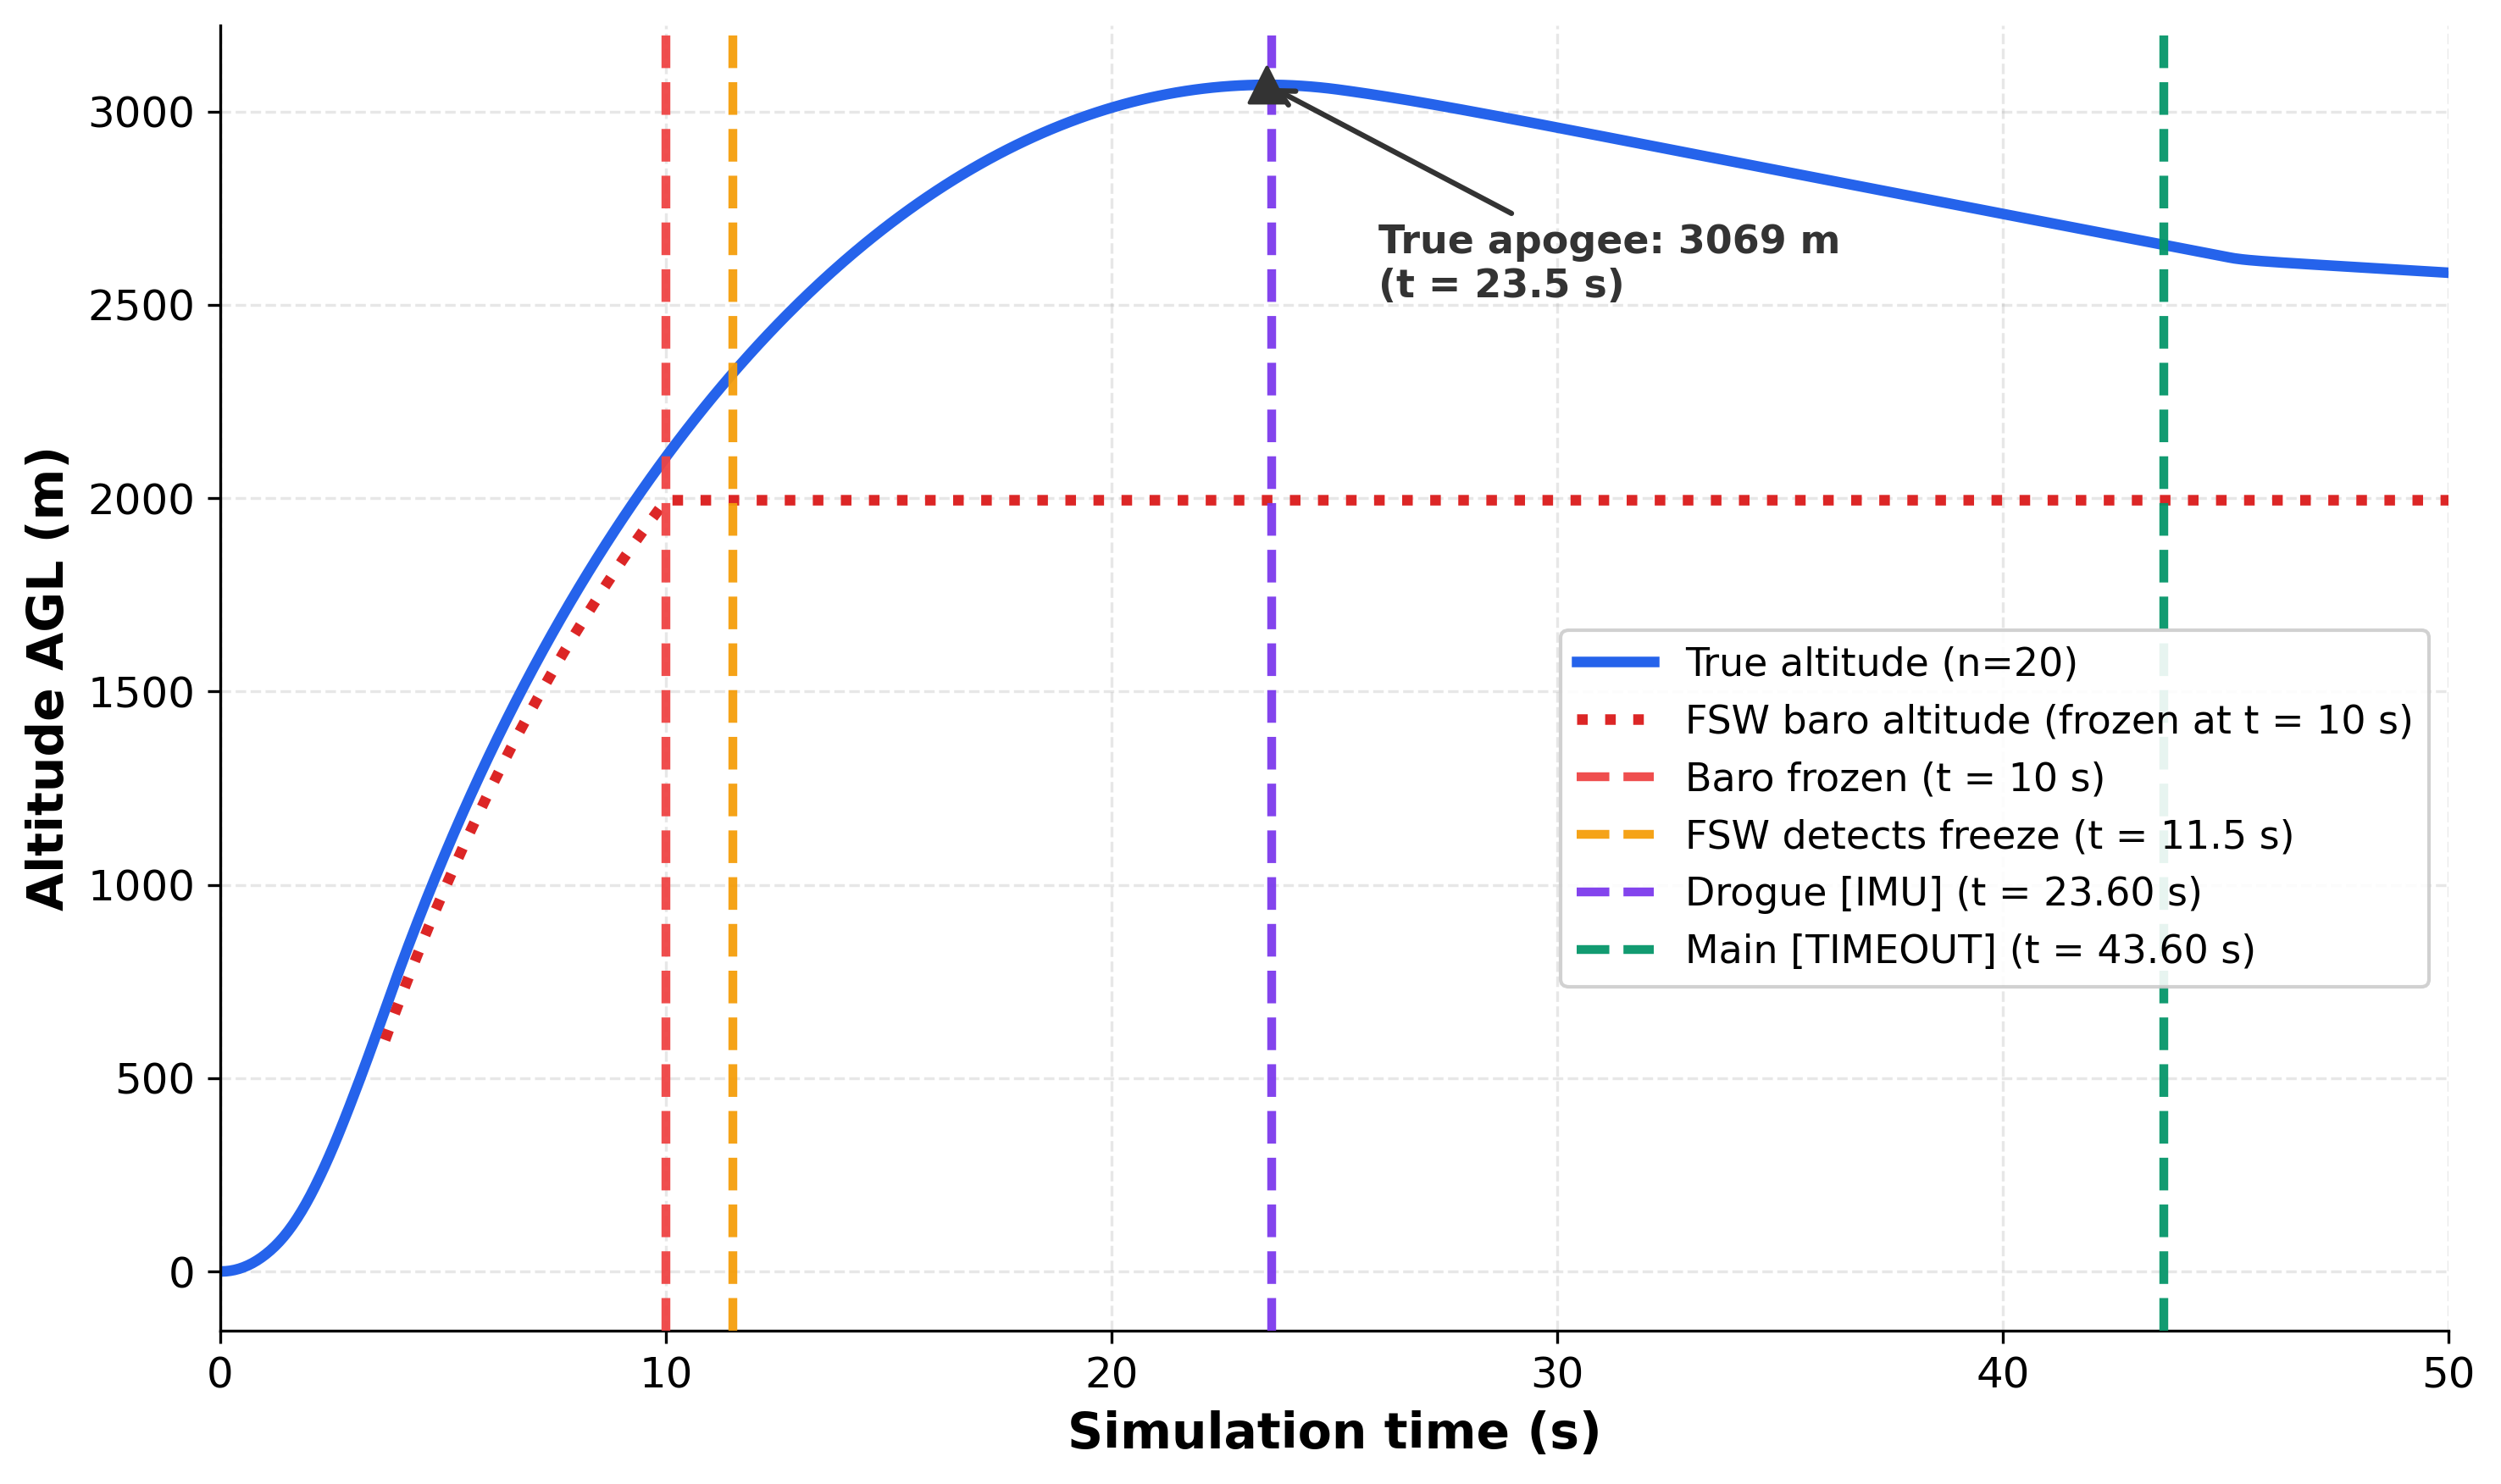
\includegraphics[width=\columnwidth]{figures/results/fault_injection.png}
    \caption{Fault injection experiment, showing the trajectory and FSW events across all 20 runs. The barometric freeze at $t$ = 10\,s triggers IMU-based fallback detection and drogue deployment 0.1 s after true apogee.}
    \label{fig:fault_injection}
\end{figure}

Notably, the IMU-based fallback logic deployed the drogue significantly closer to apogee than the nominal barometric detection. Under no-fault conditions, drogue deployment occurred 1.54\,s after apogee, while the fallback path reduced this gap by 1.44\,s.

This unintentional finding further demonstrates the value of closed-loop testing in flight software development. This result could not have been observed through open-loop testing, as it depends on the FSW to feed the actuation output back into the simulation state. The slight apogee overshoot of 3069\,m relative to the nominal Snapshot apogee of 3066\,m is a separate consequence of the barometric freeze. With altitude held constant, the \texttt{AirbrakeController} can no longer compute a valid predicted apogee, causing under-deployment of the air brakes during the coasting phase.

The difference in detection performance stems from the 10-consecutive-pressure-reading confirmation window for barometric detection. In contrast, IMU-based detection responds as soon as vertical acceleration drops below \texttt{ACCEL\_FREEFALL\_THRESH}, a condition satisfied within one callback call at apogee. The main parachute was deployed at $t=43.60$\,s in both SIL and HIL, exactly $20$\,s after drogue deployment, through the \texttt{MAIN\_DEPLOY\_TIMEOUT} fallback, confirming that the complete recovery sequence was completed under faulty-sensor conditions.

\subsection{Controller Callback Sample Rate Sweep} \label{callback-sample-rate}
Figure \ref{fig:callback-sweep-by-strategy} shows the mean apogee as a function of the controller callback sampling rate for the Non-SIL baseline, Lockstep and Snapshot strategies, with an average taken for SIL and HIL, as the two execution contexts produced near-identical results at every rate. 

Figure \ref{fig:callback-sweep-by-strategy} demonstrates that Lockstep matches the baseline closely across every tested rate (within $\sim 0.1$\,m), consistent with its zero-tick delay design, confirmed in Section \ref{coupling-results}. As expected, due to the one-tick delay, Snapshot consistently overshoots. This overshoot decreases as the sampling rate increases, from approximately 4.8\,m at 5\,Hz to 1.3\,m at 50\,Hz, with the largest reduction occurring between 10\,Hz and 25\,Hz (4.2\,m to 1.9\,m). This indicates that the one-tick delay's practical impact on apogee accuracy diminishes as the controller is invoked more frequently.

Notably, both the baseline and Lockstep show a small, shared non-monotonicity, rising slightly at 25 Hz relative to 10 Hz before decreasing again at 35 and 50 Hz. Since this appears identically in the Non-SIL baseline, which involves no coupling, Orchestrator, or FSW, it cannot be attributed to the one-tick delay or any other coupling effect. It instead reflects the PI controller's own sensitivity to discretisation at different sampling rates.

A brief check of solver time-step sensitivity found apogee remaining within 0.1\,m of the default across time steps of 0.001, 0.005 and 0.01 s for both the Non-SIL baseline and Snapshot, with wall-clock time decreasing as the step widened. A single run at a much finer step of 0.0001 s increased wall-clock time considerably, rising to 237\,s, but produced only a marginal apogee change (3066.8 m versus 3066.0 m), suggesting the one-tick delay has negligible sensitivity to the solver computational load within the range tested. A fuller repeated sweep was outside the scope of this study.

\begin{figure}[h]
    \centering
    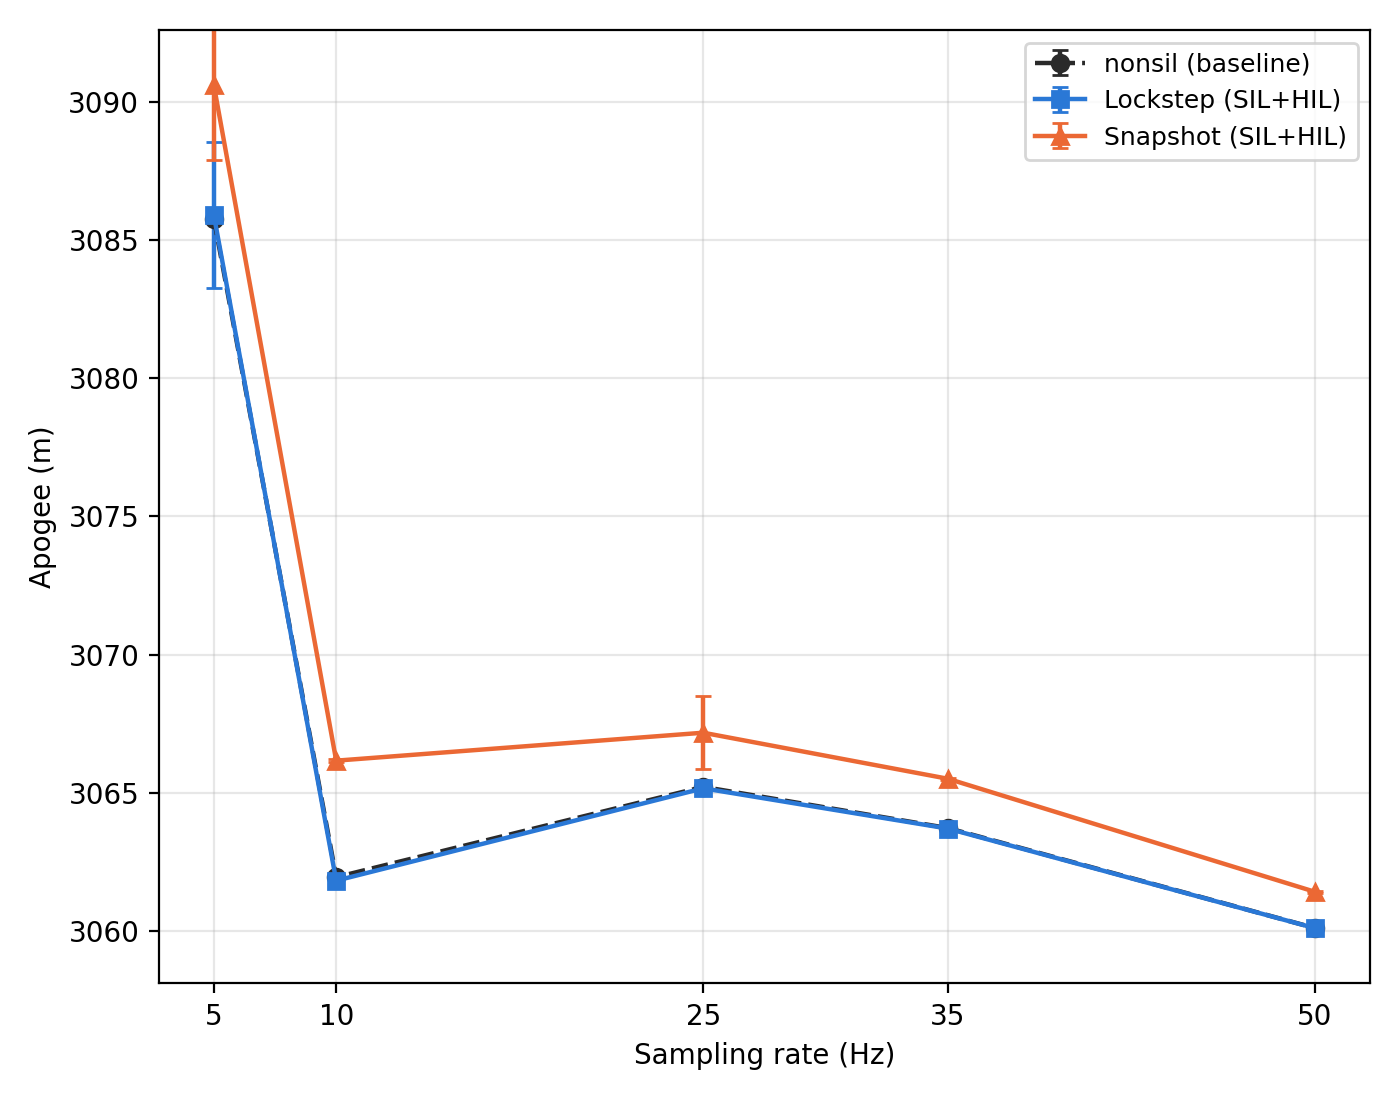
\includegraphics[width=\columnwidth]{figures/results/apogee_by_strategy.png}
\caption{Mean apogee as a function of controller callback sampling rate for the Non-SIL baseline, Lockstep and Snapshot strategies (SIL and HIL combined).}    \label{fig:callback-sweep-by-strategy}
\end{figure}



These results answer RQ2 and RQ3. Coupling strategy and execution context measurably affect apogee accuracy, deployment timing and wall-clock overhead ($H_1$, $H_2$), yet all three strategies remain within the pre-flight acceptance threshold of 12\,m in both SIL and HIL. The fault injection results confirm $H_3$: the framework successfully injects a representative sensor fault, and the FSW recovers in both execution contexts.

% \begin{table}[h]
% \centering

% \label{tab:ttest}
% \small
% \begin{tabular}{lrrr}
% \toprule
% \textbf{Comparison} & \textbf{$t$} & \textbf{$p$} & \textbf{Significant} \\
% \midrule
% Baseline vs SIL Lockstep       &   6.311  & 0.0001   & Yes \\
% Baseline vs HIL Lockstep       &   7.139  & 0.0001   & No  \\
% Baseline vs SIL Snapshot       & $-$393.6 & $<$0.001 & Yes \\
% Baseline vs HIL Snapshot       & $-$218.1 & $<$0.001 & Yes \\
% Baseline vs SIL Rate Group 25\,Hz & $-$63.8 & $<$0.001 & Yes \\
% Baseline vs HIL Rate Group 25\,Hz & $-$3.132 & 0.012  & Yes \\
% \bottomrule
% \end{tabular}
% \caption{Welch $t$-test results comparing each coupling strategy against 
% the standalone baseline. Significance assessed at $\alpha = 0.05$.}
% \end{table}






% \begin{figure}[h]
%     \centering
%     \includegraphics[width=\columnwidth]{figures/results/parachute_timing.png}
%     \caption{Drogue and Main trigger time per coupling strategy.}
%     \label{fig:drogue-timing}
% \end{figure}



% \subsection{Architecture Comparison (RQ1 \& RQ2)}

% Table~\ref{tab:summary} reports mean apogee and wall-clock time across ten runs per mode, relative to the standalone RocketPy baseline of 3061.89~m. Figure~\ref{fig:apogee_bars} shows apogee per mode and Figure~\ref{fig:wall_time} shows wall-clock 
% time distributions.

% \subsubsection{RQ 1: Accuracy}
% The lockstep architecture is the closest in similarity to the baseline in both execution contexts. SIL Lockstep produces a mean apogee of 3061.86~m, and HIL Lockstep 3061.87~m, resulting in errors of just $-0.03$ and $0.02$~m respectively. 

% Snapshot architecture produces a consistent overshoot of approximately 4.1~m in both SIL and HIL, with 

% \subsection{SIL Vs HIL (RQ3)}
% \subsection{Rate Group Frequency Sensitivity (RQ4)}
% \subsection{Fault Injection and Recovery (RQ5)}
% \TODO{
% Discuss the design of your experiments, the results you obtained, and how they
% help in evaluating the claims you made in the introduction. You may also use the
% evaluation results in this section to justify your design choices or assess the
% contributions of different aspects  of your design towards the overall goals.
% }




\section{Implications and Limitations}\label{discussion}
This section discusses implications for student rocketry teams and identifies the limitations of this study.

% \subsection{Interpretation of Results}
% \subsubsection{Non-blocking Orchestrator one-tick delay}
% The apogee overshoot observed in both the Snapshot and Rate Group strategies is a structural property of the non-blocking Orchestrator design. At callback $n$, the Orchestrator sends the current sensor packet to the FSW and immediately returns the actuation value computed at callback $n-1$ from the actuation buffer, without waiting for the FSW to process the packet from callback $n$. The actuation response corresponding to callback $n$ is therefore not applied until callback $n+1$, producing a one-tick delay, where the actuation applied at any callback is always one step behind the sensor reading that triggered it. This delay directly affects the \texttt{AirbrakeController}, as the predicted apogee estimate and the air brake deployment level are always one step behind the true simulation state, causing the PI controller to under-correct during the coasting phase and leading to a systematic overshoot. These results confirm $H_1$. 

% All three strategies remain well within the 12\,m acceptance threshold defined in Section~\ref{ss:rqs}, confirming that each is suitable for pre-flight validation despite their architectural differences. The nature of this delay was further confirmed by running the framework against a second rocket configuration, in which the overshoot magnitude differed, but the delay persisted across both non-blocking strategies, confirming that it is a property of the Orchestrator design rather than the rocket configuration. 

% The timing behaviour produced by this delay is representative of real embedded flight software execution. On real hardware, sensor readings will always be slightly stale by the time they are processed on a fixed hardware clock. Although both strategies share this behaviour, the source of the delay differs. In Snapshot, it arises from the non-blocking Orchestrator, while in Rate Group, it additionally arises from the mismatch between the two independent clocks, which is why Rate Group shows higher variance than Snapshot in both SIL and HIL contexts, most prominently in HIL. Lockstep, on the contrary, represents an idealised synchronisation model that does not exist in real hardware interacting with its environment.

% \subsubsection{Wall-clock time and execution overhead}
% It is evident from Table \ref{tab:summary} and Figure \ref{fig:wall_time_violin} that HIL configurations are slower than their SIL counterparts. For Lockstep, the overhead is most notable in both contexts due to its blocking nature. The additional cost in HIL relative to SIL (48.8\,s versus 44.9\,s) is attributable to the Ethernet round-trip between the host and the Raspberry Pi 4, as well as the reduced CPU performance of the target hardware, extending the processing time of the FSW. For the Snapshot and Rate Group strategies, neither blocks the simulation, so the additional overhead is attributed to just the Ethernet transmission latency, as reflected in the smaller but consistent gap in wall-clock times. These results confirm $H_2$: HIL configurations produce longer wall-clock times than their SIL counterparts, attributable to Ethernet latency and reduced CPU performance on the target hardware.

% \subsubsection{Rate Group Frequency Sweep}
% The Rate Group frequency sweep confirms that apogee error decreases monotonically with tick frequency, from 209\,m at 1\,Hz to 4.1\,m at 50\,Hz. At higher tick frequencies, the FSW reads more recent sensor data and actuates more frequently, reducing the window of stale data between ticks and allowing the \texttt{AirbrakeController} to track the trajectory of the rocket with higher accuracy. The diminishing accuracy gains and extra cost beyond 25\,Hz informed the selection of this frequency for the comparison of coupling strategies in Section~\ref{s:evaluation}.

% \subsubsection{Fault Injection} \label{sec:fault_inj}
% Following fault injection illustrated in Figure \ref{fig:fault_injection}, the \texttt{RecoveryController} detected the barometric freeze at $t=11.5$\,s and switched to IMU-based free-fall detection. The drogue parachute was deployed at $t=23.60$\,s in SIL and $t=23.61$\,s in HIL, approximately $0.1$\,s after apogee at $t=23.5$\,s. These results confirm $H_3$. The FSW successfully detected the sensor fault and deployed the drogue parachute near apogee in both execution contexts. 

% Notably, the IMU-based fallback logic deployed the drogue significantly closer to apogee than the nominal barometric detection. Under no-fault conditions, drogue deployment occurred 1.54\,s after apogee, while the fallback path reduced this gap by 1.44\,s.

% This unintentional finding further demonstrates the value of closed-loop testing in flight software development. This result could not have been observed through open-loop testing, as it depends on the FSW to feed the actuation output back into the simulation state. The slight apogee overshoot of 3069\,m relative to the nominal Snapshot apogee of 3066\,m is a separate consequence of the barometric freeze. With altitude held constant, the \texttt{AirbrakeController} can no longer compute a valid predicted apogee, causing under-deployment of the air brakes during the coasting phase.

% The difference in detection performance arises from the confirmation window of 10 consecutive pressure readings for barometric detection. In contrast, IMU-based detection responds as soon as vertical acceleration drops below \texttt{ACCEL\_FREEFALL\_THRESH}, a condition satisfied within one callback call at apogee. The main parachute was deployed at $t=43.60$\,s in both SIL and HIL, exactly $20$\,s after drogue deployment, through the \texttt{MAIN\_DEPLOY\_TIMEOUT} fallback, confirming that the complete recovery sequence was completed under faulty-sensor conditions.

% Together, these results answer RQ2 and RQ3. Coupling strategy and execution context measurably affect apogee accuracy, deployment timing and wall-clock overhead ($H_1$, $H_2$), yet all three strategies remain within the pre-flight acceptance threshold of 12\,m in both SIL and HIL. The fault injection results confirm $H_3$: the framework successfully injects a representative sensor fault, and the FSW recovers in both execution contexts.

\subsection{Implications for Student Rocketry Teams} \label{implications}
The primary audience for RITL is university rocketry teams operating under the constraints of limited budgets, part-time contributors and single-use rockets, where a software fault during flight cannot be corrected. 



%The result of this study suggests that RITL is a practical tool for this context.

To assess practical accessibility, the framework was informally trialled as part of a recruitment exercise for the RISE student rocketry team, in which prospective members were evaluated for selection in the following year. Participants were provided with an RITL deployment, including a base implementation of the FSW that connects to RocketPy and were tasked with independently implementing parachute deployment and air brake control logic. The trial was conducted in SIL only. Participants successfully executed SIL runs with accurate parachute deployments and control logic, suggesting that the framework is accessible to newcomers without prior knowledge of the internals. A controlled usability study across multiple teams would be needed to substantiate this claim more rigorously.

The choice of coupling strategy should reflect the validation goal. Lockstep is best suited for validating flight logic correctness under ideal conditions, particularly control algorithm behaviour, as its tight synchronisation eliminates actuation delay and produces an idealised closed-loop response similar to model-based validation tools such as Simulink. The advantage over such tools is that the software under test is the actual flight software that will fly, not a model of it. There are no code generation steps, no reimplementation of flight logic from block diagrams and no fidelity gap introduced by translating a validated model into a deployed binary.

Snapshot and Rate Group strategies are more suited for timing validation, as both reproduce the one-tick actuation delay that is analogous to real embedded execution. Snapshot is the simpler of the two and serves as a middle ground. Rate Group goes further by running the FSW on an independent hardware timer, making it most useful for characterising how timing non-determinism affects performance before launch. 

The Rate Group tick frequency is not a parameter unique to RITL. Real flight computers already run their control loop at a fixed frequency, chosen by the team based on what their hardware can sustain alongside its other responsibilities. Teams should configure \texttt{RateGroupDriver} to the frequency they have already selected or plan to select for their real flight computer. This ensures that pre-flight validation reflects the actual rate at which recovery logic will execute in flight.

The same principle extends to the other timing parameters RITL exposes: the controller callback rate, the sensor model sampling rate, the parachute trigger rate and the solver's integration time step. The controller callback rate, the Rate Group tick frequency and the parachute trigger rate conceptually represent the same underlying quantity, the frequency of the flight computer's control loop. Since \texttt{AirbrakeController} and \texttt{RecoveryController} both execute within that same loop on real hardware (Section~\ref{flight-logic}), all three should therefore be matched to whatever loop frequency the team's real flight computer runs at. However, RocketPy registers the air brake and parachute callbacks independently, so RITL does not currently enforce this correspondence. In this study, both were held equal at 10 Hz by configuration choice. The sensor model sampling rate instead corresponds to the physical sensor's own output rate, typically specified in its datasheet, and should be matched to that value. The solver's integration time step has no equivalent on real hardware at all, as the physical rocket's flight is continuous rather than stepped. It should instead be chosen fine enough to keep the underlying physics accurate, independent of the target flight computer.

By design, the Orchestrator architecture also lowers the barrier to HIL testing. Since the SIL-to-HIL transition requires no changes to the Orchestrator or flight software beyond recompiling the F Prime deployment for the target hardware, teams could in principle validate their software on actual flight hardware without building expensive test infrastructure. This claim follows from the framework's architecture described in Section~\ref{closed-loop-sim-env} rather than from empirical trial data, since the informal trial above was conducted in SIL only. 

The fault injection capability adds another dimension that is otherwise difficult to test before launch. By having a dedicated fault injection interface in the Orchestrator, teams can apply any sensor fault pattern to the simulation without modifying the FSW, testing recovery logic against failure modes that would otherwise only be discovered during flight.


Finally, the Orchestrator design decouples flight software from the simulator, allowing either to be replaced independently without modifying the other side of the interface. Teams that switch trajectory simulators, upgrade their FSW framework, or retarget to different hardware need only update the relevant side of the coupling.

These architectural properties and the positive outcome of the SIL trial suggest RITL is a practical tool for student rocketry teams.

\subsection{Limitations} \label{limitations}
The following limitations concern constraints in the current implementation and experimental scope, rather than the validity of the reported results, which are addressed separately in Section~\ref{sec:threats}.


% The communication layer between the Orchestrator and the FSW uses TCP in both SIL and HIL execution contexts. An alternative would be UDP, which removes the connection overhead and more closely represents the non-acknowledged transport behaviour of real embedded systems. This would also likely reduce wall-clock time in both execution contexts.

The fault injection experiment targets only the \texttt{RecoveryController}. The \texttt{AirbrakeController} did not implement fallback logic. When tested with a barometric freeze, it held onto the last predicted apogee estimate, causing under-deployment of the air brakes and the overshoot observed in the fault injection results.

% The RocketPy callback rate is fixed at 10\,Hz across all experiments. This rate determines the precision of the simulation loop and directly affects the one-tick delay observation. The sensitivity of the results to this parameter was not evaluated; thus, running the framework at different callback rates would clarify how this design choice affects coupling accuracy across strategies.

The \texttt{MAIN\_DEPLOY\_DELTA\_HPA} threshold is configured to deploy the main parachute approximately 330\,m below apogee, resulting in the main parachute deployment at approximately 2700\,m AGL across all coupling strategies. This does not reflect a typical competition deployment altitude and was not optimised for a specific use case, as the flight software in this study serves as a validation system for the closed-loop framework rather than a production-ready flight computer.

The PI controller was not formally tuned. The constants were selected to produce stable actuation sufficient to exercise the coupling strategies. Any difference between the achieved apogee and the 3000 m target is consistent across all configurations, as the same controller is used in both the baseline and RITL setups, and therefore does not affect the coupling strategy comparison.

The solver time step sensitivity check in Section \ref{callback-sample-rate} was evaluated with a single run per time step, rather than the 10 runs used in the rest of the study. This was a scope reduction given its exploratory purpose and the considerably higher wall-clock cost of the finest step tested. The results were sufficient to show that apogee was not sensitive to step size within the range tested, but a fuller sweep could characterise this relationship more accurately.


\section{Threats To Validity}\label{sec:threats}

This section assesses the internal, external, construct and conclusion validity of the study's design and results.

\subsection{Internal Validity}
% did x cause y or something else
The comparative baseline in this study is a standalone RocketPy simulation in which the flight logic, including the PI controller, apogee detection and parachute deployment, is directly reimplemented into the controller callback. Any difference between this reimplementation and the F Prime flight software would cause the measured apogee difference to be due to an implementation discrepancy rather than a pure coupling strategy effect. The baseline was constructed to match the F Prime logic as closely as possible, but the two are not formally equivalent.


\subsection{External Validity}
% do results generalise beyond this study
Aside from the informal check against a second rocket configuration in Section \ref{coupling-results}, all experiments were conducted on a single fixed rocket configuration, with a fixed motor, geometry and target apogee of 3000\,m. The quantitative results observed in this study, such as the overshoot in non-blocking strategies, wall-clock overhead, and fault detection timing, are specific to this configuration. Evaluating RITL across rockets with different coasting durations, apogee targets, and aerodynamic profiles would be needed to characterise how the accuracy of the coupling strategy scales across mission types.

% The fixed 10\,Hz callback rate used in RocketPy across all experiments is a design choice, not a result. The one-tick delay identified in Section~\ref{s:evaluation} is a function of this rate, as the magnitude of overshoot will vary at different callback frequencies. The conclusions about the Snapshot and Rate Group accuracy are thus specific to this configuration.

The controller callback rate and the Rate Group tick frequency were both varied experimentally in this study on the same fixed rocket configuration used throughout. The specific error magnitudes reported at each rate are therefore not guaranteed to generalise to different rockets. The sensor model sampling rate and the parachute trigger rate were additionally held fixed throughout and were not varied experimentally, so whether they exhibit a similar relationship remains untested.

The fault injection experiment evaluates a single fault type: a barometric freeze at $t=$10\,s. Other fault modes, such as sensor drift, noise or dropout, could trigger different recovery paths or expose failures not addressed in this study.

The HIL target in this study is a Raspberry Pi 4 running standard RPi OS, without real-time scheduling guarantees. While F Prime supports deployment on bare-metal and RTOS-based microcontrollers, the timing behaviour observed in HIL reflects the behaviour of that platform. Teams deploying on different embedded targets, such as STM32 or similar, may observe different results. The communication layer further limits this generalisability. The Orchestrator and FSW communicate over TCP, routed over Ethernet in HIL, chosen since Lockstep requires reliable delivery. Real flight computers typically read sensors over SPI or UART, unacknowledged communication operating at lower latency than TCP over Ethernet. The wall-clock times and timing variance reported in HIL are therefore specific to this transport configuration, and a lower-latency, unacknowledged link would likely reduce both wall-clock overhead and the practical impact of the one-tick delay.



\subsection{Construct Validity}
% did we measure the right thing

The primary measures of coupling accuracy in this study are apogee error and deployment timings, which are measured relative to the standalone RocketPy baseline. This has two limitations. First, the reference is itself a model, so the apogee differences reported in this study are relative to a modelled trajectory, not a real flight, and the true accuracy of any coupling strategy against an actual flight using the same FSW remains uncharacterised.

Second, while this study adopts a 12\,m acceptance threshold derived from the Camões configuration, acceptable tolerances beyond this bound depend on the specific rocket, target apogee and mission requirements. The results reported in this paper characterise the error introduced by each coupling strategy, but whether that error is significant is mission-dependent.

\subsection{Conclusion Validity}

%do the statistics support the claims
Each configuration was evaluated over 10 runs. For Lockstep and Snapshot strategies, where variance is low, this is sufficient to support the results drawn. For the Rate Group strategy in HIL, which produces a standard deviation of 7.46\,m at 25\,Hz, 10 runs limit the coverage of the distribution. The worst-case apogee error under such timing non-determinism could exceed the observed mean, and a larger sample would be required to characterise this with more confidence. The solver time step sensitivity check is an exception, evaluated with a single run per step size given its exploratory scope. This is discussed further in Section \ref{limitations}.

\section{Conclusion}\label{s:conclusion}
Answering RQ1, this thesis presented RITL (Rocket in the Loop), a closed-loop framework that couples the RocketPy flight simulator with the F Prime flight software framework via a dedicated Python Orchestrator. RITL is the first framework to couple these two tools in a closed feedback loop, enabling flight software to receive sensor input and return actuation output that influences the simulation state at each step. The framework supports SIL and HIL execution, three coupling strategies and fault injection within the simulation loop, directly addressing a gap that existing open-loop HPR tools could not fill. 

Addressing RQ2, three coupling strategies span from fully synchronised to fully decoupled. Lockstep, which blocks at every callback until the FSW responds, produces a mean apogee within 0.08\,m of the standalone baseline in both SIL and HIL execution contexts. This makes it the most accurate strategy to validate the flight logic correctness under ideal conditions. Snapshot and Rate Group strategies produce a one-tick actuation delay, which directly arises from their non-blocking Orchestrator design. Snapshot produces a consistent 4.1\,m overshoot, while Rate Group's overshoot ranges from 3.84\,m (SIL) to 7.39\,m (HIL), reflecting additional timing non-determinism. A frequency sweep of the Rate Group strategy showed that apogee error decreases monotonically with tick frequency from 209\,m at 1\,Hz to 4.02\,m at 50\,Hz, with diminishing accuracy gains beyond 25\,Hz, informing the selection of this frequency for the strategy comparison. HIL configurations introduce additional wall-clock overhead relative to their SIL counterparts, attributable to Ethernet round-trip latency and the reduced CPU performance of the Raspberry Pi 4 target.

A sweep of the controller callback rate under the Lockstep and Snapshot strategies showed the same trend: Lockstep matched the baseline within approximately 0.1\,m at every tested rate, while Snapshot's overshoot fell from 4.8\,m at 5\,Hz to 1.3\,m at 50\,Hz. A brief check of solver time-step sensitivity found no meaningful effect on apogee within the range tested.

For RQ3, the fault injection experiment demonstrated that the FSW successfully detected a simulated barometric freeze mid-flight and completed the full recovery sequence in both SIL and HIL contexts. Notably, the IMU-based fallback was deployed within 0.1\,s of apogee, compared to 1.54\,s under nominal barometric detection, a result that could not have been observed through open-loop testing alone, and one that further demonstrates the value of RITL for flight software development.

Future work should evaluate UDP as a replacement for TCP between Orchestrator and F Prime, which should reduce communication overhead and more closely reflect embedded transport behaviour. Extending the fault injection coverage to include air brake fallback logic, additional faults, and a broader range of rocket configurations would strengthen the generalisability of the results. Deploying and running the framework on a bare-metal or RTOS-based target would address the timing constraints that the Raspberry Pi 4, running a standard OS without real-time scheduling guarantees, could not fully capture. Finally, generalising the simulator side of the Orchestrator and adding an interface for a standard Functional Mock-up Unit (FMU) would decouple the framework from RocketPy specifically, allowing any FMI-compliant simulator, such as Simulink, to be coupled with F Prime through the same interface. This would align RITL with established co-simulation tooling used in industry, broadening the range of compatible simulators and lowering the barrier for teams already invested in existing simulation environments to adopt a closed-loop testing workflow.

Student rocketry teams now have a tool that did not exist before: a closed-loop environment in which the actual flight software, not a model of it, is run against a physics-based trajectory simulation before a rocket ever leaves the pad. As missions grow more ambitious and flight software more complex, the need for this kind of pre-flight validation will only increase. RITL is a step toward making that infrastructure accessible to teams that cannot afford to learn from a failed launch.

%future work : controlled experiment testing development with and withou RITL

%maybe move implications to section 6
% move answering RQ to discission









\bibliographystyle{IEEEtran}
\bibliography{references}


\end{document}
